
\chapter[Fundamentação Teórica]{Fundamentação Teórica}

Dando continuidade à discussão sobre sistemas autônomos nos processos produtivos, pode-se citar que são 
vários os benefícios conquistados pelas empresas e por seus clientes ao se utilizar essa abordagem: 


\begin{itemize}

	\item Redução de custos: Sistemas automatizados são capazes de reduzir custos de maneira significativa a 
curto prazo por meio do aumento de produtividade e eficiência;
	\item Qualidade: Máquinas autônomas fornecem resultados consistentes e repetíveis, sendo que, os problemas
 de controle de qualidade envolvidos como o erro humano são totalmente eliminados. Além disso, os processos podem 
ser cuidadosamente regulados e controlados de acordo com a necessidade do empresário;
	\item Segurança: Como já apresentado, sistemas automatizados estão praticamente imunes aos erros que 
um operador humano possa vir a cometer, caso estivesse realizando o seu trabalho. Sistemas automatizados industriais 
devem possuir a premissa de segurança fornecidas pelas normas regulamentadoras, que estão em vigor no país em questão;
	\item Monitoramento remoto: Sistemas de automação e de informatização oferecem a vantagem de permitir ao 
operador monitorar e/ou controlar os processos de produção fora do seu local de implantação. Dependendo da estrutura 
adotada e da implementação, esse monitoramento pode ser feito em tempo real.

\end{itemize}


Conforme apresenta \cite[p.~87]{barreto1993}, um sistema supervisório é constituído por uma plataforma computacional, 
que integra a análise de diversas transações de troca de informação e sinais entre um sistema de computação e um processo, 
de modo a obter um diagnóstico da evolução dos estados do sistema, atuando também sobre estes dados nos casos onde isto se 
faça necessário. Um modelo básico de um sistema supervisório é representado de acordo com a \autoref{supervisorio}.

\begin{figure}[h]
	\centering
	\caption{\label{supervisorio}Estrutura básica de um sistema supervisório.}
		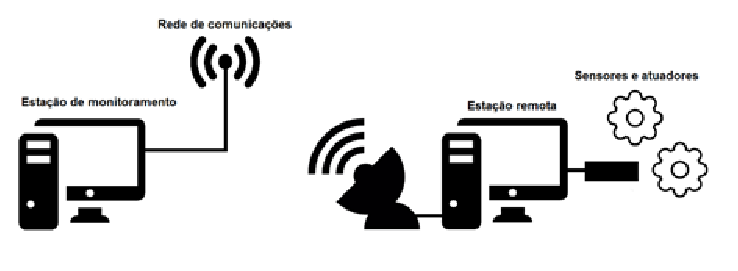
\includegraphics[keepaspectratio=true,scale=1]{figuras/supervisorio.eps}
	\fonte{Autoria própria.} % Referencia errada
\end{figure}

O sistema apresentado na \autoref{supervisorio} é também conhecido como \texttt{SCADA (Sistemas de Controle de Supervisão e Aquisição de Dados)} 
sendo que, a sua implementação irá depender da arquitetura de redes industriais utilizada. Na \autoref{supervisorio}, a estação de trabalho 
é responsável por armazenar o \textit{software} de gerenciamento do \texttt{SCADA}, a rede de comunicações pode ser implementada de várias maneiras 
como: cabeamento \texttt{ethernet}, \texttt{bluetooth}, rádio frequência, entre outras. A estação remota é geralmente composta por algum microcontrolador 
que recebe sinais provenientes dos sensores e envia comandos aos atuadores oriundos da estação de monitoramento. Nesse ponto é 
importante que fique claro a diferença entre microprocessadores e microcontroladores. Uma definição bastante interessante é apresentada 
por \cite{andrade2006} em que afirma que, microcontroladores assim como microprocessadores são circuitos integrados disponíveis 
nos mais variados tipos de encapsulamento, sendo destinados ao tratamento de sinais digitais. Entretanto, microcontroladores geralmente 
possuem todos os periféricos necessários num único \texttt{chip}. Microprocessadores por sua vez não conseguem realizar o seu trabalho sozinho, 
já que para o seu funcionamento é necessário a integração de outros dispositivos externos (periféricos) para que ele se torne útil.

Em muitos casos é desejável que o sistema apresentado na \autoref{supervisorio} detecte os eventos assim que ocorrerem, ou seja, de maneira praticamente 
instantânea. Para que isso seja possível é necessário a utilização de um sistema de \textit{software} que tenha suporte à execução de múltiplas tarefas 
em que o tempo de resposta a um evento seja conhecido. Independentemente do contexto, esse tempo pré-definido (conhecido também como tempo de 
resposta) deverá ser cumprido, ou seja, deverá ser determinístico. O não comprimento desse prazo é tido como uma falha de sistema. Sistemas que 
apresentam essas características são denominados sistemas de tempo real, mais conhecidos pela sigla \texttt{RTOS - Real Time Operating System}. A detecção 
de eventos nesse tipo de sistema é baseada no uso de interrupções de \textit{hardware}\footnote{Um sinal que geralmente resulta em uma troca de contextos no processador.}, sendo que o tratamento de tais interrupções irá depender do microcontrolador em questão. Esse tipo de sistema é utilizado em vários ramos da indústria, agricultura e comércio. Sua utilização está envolvida em sistemas dos mais variados níveis de complexidade e periculosidade: em coisas relativamente simples como jogos eletrônicos e videoconferências até a sistemas críticos de controle de usinas nucleares e freios automotivos. Mais informações a respeito de um \texttt{RTOS} são apresentadas nas próximas seções.

Outro aspecto importante na implementação do sistema da \autoref{supervisorio} se diz respeito a arquitetura a ser 
adotada na estação remota. Nesse contexto é importante se ter em mente os conceitos de processadores \texttt{RISC} e 
processadores \texttt{CISC}. Basicamente processadores \texttt{RISC (Reduce Instruction Set Computer)} apresentam um 
conjunto de instruções reduzido enquanto processadores \texttt{CISC} possuem um conjunto complexo de centenas de instruções. Conforme apresenta \cite[p.~1]{marimoto2007} a arquitetura \texttt{CISC} tem as seguintes vantagens:

\begin{citacao}
``[...] um processador \texttt{RISC} é capaz de executar tais instruções muito mais
rapidamente. A ideia principal, é que apesar de um processador \texttt{CISC} ser capaz de
executar centenas de instruções diferentes, apenas algumas são usadas
frequentemente. [...] é indiscutível, porém, que em instruções complexas os
processadores \texttt{CISC} saem-se melhor.''
\end{citacao}

A vantagem da arquitetura \texttt{CISC} está relacionada ao seu vasto conjunto de instruções armazenadas no processador, o que facilita o trabalho 
dos programadores, que dispõem de praticamente todas as instruções que seus \textit{softwares} farão uso. No caso de processadores \texttt{RISC}, 
\textit{softwares} mais complexos teriam que combinar uma série de instruções a fim de executar a mesma tarefa mais complexa que poderia ser executada
por apenas uma instrução \texttt{CISC}. Isso gera um maior nível de complexidade para o programador que está desenvolvendo a aplicação. 
Geralmente a estação remota é constituída por uma unidade \texttt{RISC} em função de suas operações na maioria dos casos consistirem por 
tarefas relativamente simples.


\section{Estação Remota - Possibilidades de implementação}

A estação remota é implementa utilizando-se algum tipo de microcontrolador que atenda às necessidades do projeto. 
Existem várias possiblidades quanto a modelos e marcas que podem ser utilizadas, sendo os tipos mais utilizados:
Plataforma \texttt{Arduino}, famílias \texttt{PIC}, \texttt{FPGA}, famílias \texttt{Texas Intruments}, famílias \texttt{Freescale}. 
Independente da marca e família adotada no projeto, é importante ter em mente que, o microcontrolador deverá apresentar algumas 
características globalmente desejáveis que são:

\begin{itemize}

	\item Baixo consumo energético;
	\item Baixo tempo de resposta;
	\item Baixo custo de aquisição;
	\item Alta confiabilidade;
	\item Imunidade a ruídos e interferências;

\end{itemize}

A seguir será apresentada uma breve discussão a respeito de cada um desses segmentos de microcontroladores.

\subsection{Microcontroladores \textit{PIC}}

Trata-se de uma série de circuitos integrados produzidos pela empresa \texttt{Microchip Technology Inc.}, que apresentam integrado em um único dispositivo todos os circuitos necessários ao desenvolvimento de um sistema digital programável completo. 
A principal vantagem do \texttt{PIC} em relação ao restante dos microcontroladores é devido ao fato de fazer uso da arquitetura \texttt{Harvard} que, conforme apresenta \cite[p.~27]{andrade2006}:

\begin{citacao}
``Na arquitetura de \texttt{Von Neumann} existe apenas um barramento por onde passam os
dados de memória de programa e da memória de dados, enquanto na arquitetura de
\texttt{Harvard} existem barramentos diferentes, proporcionando maior desempenho, pois
permitem múltiplos acessos à memória, ou seja, acessos simultâneos à memória de
dados e à memória de programa.''
\end{citacao}

Os microcontroladores com arquitetura \texttt{Havard} são também conhecidos como “microcontroladores \texttt{RISC}” enquanto os microcontroladores com arquitetura \texttt{Von Neumann}, de “microcontroladores \texttt{CISC}”. O alto desempenho da família de microcontroladores \texttt{PIC} pode ser atribuído as seguintes características proporcionadas pela arquitetura \texttt{RISC}:

\begin{itemize}

	\item Mapa de Registradores versátil;
	\item Todas as instruções com palavras simples;
	\item Palavra de instrução longa;
	\item Arquitetura de instruções em \textit{pipeline};
	\item Instruções de apenas um clico de máquina;
	\item Conjunto de instruções reduzido;
	\item Conjunto de instruções ortogonal (simétrico).

\end{itemize}

A \autoref{von} e \autoref{harvard} apresentam as diferenças entre as arquiteturas de \texttt{Von-Neumman} e \texttt{Havard} respectivamente:

\begin{figure}[h]
	\centering
	\caption{\label{von}Arquitetura de \texttt{Von-Neumman}.}
		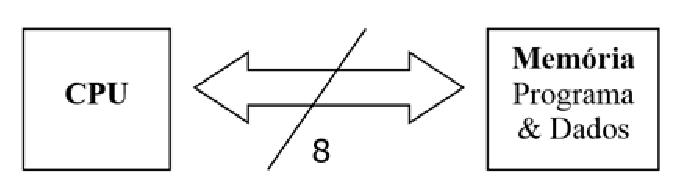
\includegraphics[keepaspectratio=true,scale=1]{figuras/von.eps}
	\fonte{Autoria própria.} % Referencia errada
\end{figure}

\begin{figure}[h]
	\centering
	\caption{\label{harvard}Arquitetura \texttt{Harvard} apresentada em um microcontrolador \texttt{PIC} (a numeração representa a quantidade de \textit{bits} do barramento).}
		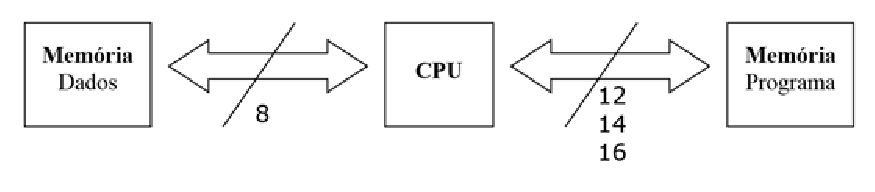
\includegraphics[keepaspectratio=true,scale=1]{figuras/harvard.eps}
	\fonte{Autoria própria.} % Referencia errada
\end{figure}

Existem várias versões de \texttt{chips} na família \texttt{PIC}, tendo modelos capazes de processar dados de 8, 12, 16 ou 32 \textit{bits}. Esses dispositivos são amplamente utilizados na indústria quanto por \textit{“hobystas”} em função do seu baixo custo, ampla disponibilidade e grande acervo de material de desenvolvimento. 
Com relação ao seu desempenho, os microcontroladores \texttt{PIC} tem a sua arquitetura implementada de forma a maximizar a relação de velocidade-custo. O seu conjunto de instruções se mostra adequado a construção de tabelas de consulta rápida, sendo que, tais consultas ocupam uma instrução e dois ciclos de instrução. 
 Apesar disso, a plataforma \texttt{PIC} está perdendo espaço para outras alternativas presentes no mercado. Isso se deve ao fato do alto custo de seu gravador (desestimulando a sua utilização em pequenos projetos) e poder de processamento insatisfatório nas versões de 8 \textit{bits} quando comparado a outros dispositivos que também trabalham com esse tamanho de palavra.

\subsection{Plataforma \texttt{Arduino}}
\label{due}

\texttt{Arduino} consiste em uma plataforma de prototipagem aberta que utiliza microcontroladores \texttt{ATMEL AVR}. Consiste em uma solução relativamente recente no mercado, tendo sido criada em 2005 com o objetivo de servir como base para projetos de baixo custo. Utiliza o mesmo conjunto de instruções reduzido de instruções \texttt{(RISC)} utilizado nos dispositivos \texttt{PIC}. Sua principal característica é a simplicidade, que faz com que seja bastante popular no meio dos desenvolvedores amadores e experientes; sua utilização não requer conhecimentos avançados de eletrônica.

Essa ideia é reforçada por \cite[p.~3]{vasiljevic2013} apresentando que:

\begin{citacao}
``O \texttt{Arduino} foi criado com o propósito de ser uma plataforma extremamente fácil de
usar se comparado às outras [...] Outro fator que torna o \texttt{Arduino} atrativo é sua
filosofia de \textit{hardware} livre, ou seja, pessoas podem usá-lo para criar diversos projetos
sem custo algum de direitos pela utilização da plataforma [...].''
\end{citacao}

Dentre as soluções apresentadas para o desenvolvimento de uma estação remota de um sistema \texttt{SCADA}, o \texttt{Arduino} é a que apresenta a documentação mais diversificada e acessível, contando com milhares de comunidades na internet de pessoas que divulgam informações e detalhes dos projetos que criam. O campo de aplicações de tal plataforma é ilimitado. A \autoref{arduino} apresenta o diagrama de blocos simplificado de um \texttt{Arduino}.


\begin{figure}[h]
	\centering
	\caption{\label{arduino}Diagrama de blocos simplificado de um \texttt{Arduino}.}
		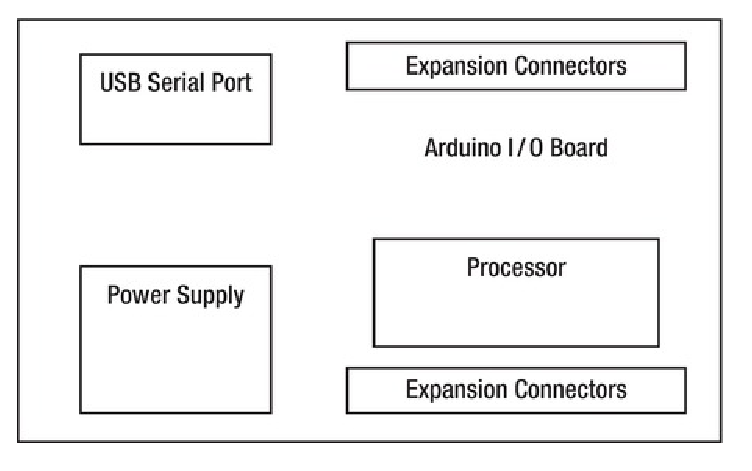
\includegraphics[keepaspectratio=true,scale=1]{figuras/arduino.eps}
	\fonte{\cite[p.~2]{wheat}.} % Referencia errada
\end{figure}

Existem diferentes versões de \texttt{Arduino}, como a \texttt{UNO}, \texttt{MEGA}, \texttt{LEONARDO}, \texttt{DUE}, \texttt{MEGA ADK}, \texttt{NANO}, \texttt{MINI} e \texttt{ESPLORA}. A versão a ser adotada irá depender das características do projeto. A grande maioria de suas versões são baseadas no chip \texttt{ATmega8} e seus derivados. Informações detalhadas a respeito de cada versão podem ser encontradas no livro \texttt{“Arduino Internals”} escrito por \texttt{Dale Wheat}. O núcleo do \texttt{Arduino} processa dados de 8 ou 32 \textit{bits}, sendo está última versão destinada a projetos que requerem maior poder de processamento. A versão \texttt{DUE} é a que apresenta maior poder de processamento sendo baseada em um núcleo \texttt{ARM Cortex-M3} que funciona até 84 \textit{MHz}. As demais versões de 8 \textit{bits} trabalham com um \textit{clock} de até 16 \textit{MHz}.

\subsection{Microcontroladores \textit{Freescale}}

A fabricante \texttt{Freescale Semiconductor, Inc.} possui uma diversificada linha de microcontroladores, sendo o seu foco a área de sistemas embarcados e comunicação. Sua linha atual de projetos são todos baseados na arquitetura \texttt{ARM}. Atualmente a empresa tem o seu foco na família de microcontroladores \texttt{Kinetis} e na plataforma de desenvolvimento \texttt{Freedom} que utiliza os núcleos dessa família.
As placas \texttt{Freedom} são equipadas com microcontroladores \texttt{Kinetis} e são uma forma rápida, prática e barata para os primeiros contatos com os dispositivos desenvolvidos pela empresa. A placa já vem com alguns dispositivos integrados como \textit{touch pad}, sensor infravermelho, termistor, conectores compatíveis com \textit{shield} \texttt{Arduino R3}, entre outros. Por se tratar de uma plataforma de desenvolvimento com vários periféricos integrados, apesar do seu baixo custo, sua utilização pode não ser viável em alguns tipos de projeto. A linha \texttt{Freedom} é baseada no núcleo \texttt{ARM Cortex-M0+} ou no \texttt{ARM Cortex-M4}, conforme cita \cite{lima} em seu site, tais unidades baseadas no \texttt{Cortex-M0+} implementam a arquitetura de \texttt{Von Neumann} sendo microcontroladores de 32 \textit{bits} de baixo custo desenvolvidos pela \texttt{ARM}, que tem por objetivo ocupar o lugar de microcomputadores bem simples que realizam funções especificas ou que demandam baixo consumo de energia. O núcleo funciona com uma velocidade de \textit{clock} de até 48 \textit{MHz}. Entre as novidades apresentadas pela linha \texttt{Freedom}, destacam-se a implementação de dois estágios de \textit{pipeline} o que diminui os acessos feitos pelo processador à memória \textit{flash}, consequentemente, diminuindo o consumo da unidade central. As interrupções possuem uma latência menor em relação a outros núcleos, proporcionando um tempo de chamada de função bem pequeno o que o torna bastante interessante a aplicações em \texttt{RTOS}. Além disso foi implementado um sistema de unidade protegida de memória em que há suporte a execução em nível de privilégio ou não privilegiado. As unidades baseadas no núcleo \texttt{Cortex-M4} além das características já citadas, apresentam maior custo e poder de computação, podendo operar a até 120 \texttt{Mhz}.  Além disso, as unidades \texttt{Cortex-M4} apresentam maiores quantidades de memória \texttt{RAM} e memória \texttt{flash}.

\subsection{Microcontroladores \texttt{Texas Instruments}}

A \texttt{Texas Instruments} é uma empresa que atua na área de semicondutores oferecendo as mais variadas soluções na área de 
microcontroladores \texttt{DSPs}, conversores \texttt{A/D} e \texttt{D/A}. Dentre as centenas de modelos oferecidos pela empresa, 
atualmente a sua melhor relação custo-benefício para implementação de sistemas supervisórios são os microcontroladores da linha 
\texttt{MSP430} já que reúne praticidade e simplicidade de aplicação com um custo acessível. Conforme apresenta o \cite{sabereletronica} 
essa nova família apresenta baixo consumo de corrente, combinado com periféricos inteligentes e integrados, sendo que o \texttt{MSP430} é 
ideal para aplicações de baixo custo, incluindo equipamentos industriais e médicos portáteis, medição inteligente e aparelhos eletrônicos 
de consumo, assim como uma ampla gama de novas aplicações. Esse dispositivo utiliza a arquitetura \texttt{RISC} de 16 \textit{bits}. Os membros 
dessa família diferem entre si em questões relacionadas à quantidade memória \textit{flash} e memória \texttt{RAM} além dos periféricos 
integrados disponíveis. A \texttt{CPU MSP430} vem equipada com um conjunto de apenas 51 instruções (sendo 27 físicas e 24 emuladas) e um total 
de 16 registradores de 16 \textit{bits}. Essa \texttt{CPU} trabalha com um \textit{clock} de até 16 \textit{MHz} e atualmente é uma forte 
concorrente da plataforma \texttt{Arduino}.

\section{Sistemas Operacionais de Tempo Real, Interrupções e \texttt{I/O} Programada} 
Conforme apresenta \cite[p.~473]{limaevilaca} um sistema operacional – \texttt{SO} é definido como sendo: 

\begin{citacao}
``[...] uma coleção de programas que atua como uma interface entre programas do usuário e o \textit{hardware}. Sua principal função é proporcionar um ambiente para que o usuário de um sistema microprocessado execute programas no \textit{hardware} do sistema de uma maneira conveniente e eficiente.``
\end{citacao}

O \texttt{SO} é o responsável pelo gerenciamento do processador, da memória e dos dispositivos de entrada e saída do sistema. A partir disso é fácil concluir-se a grande complexidade envolvida em sua implementação; isso vale mesmo em \texttt{SO’s} relativamente simples como por exemplo os embarcados em fornos micro-ondas, máquinas de lavar e robôs que se quer possuem interface gráfica.  A diferença básica entre um sistema operacional e uma aplicação convencional está na maneira em que as rotinas são executadas. Sistemas operacionais tem suas rotinas executadas concorrentemente em função de eventos assíncronos. A \autoref{so} apresenta a visão geral de um sistema operacional e o seu posicionamento nessa topologia. 

\begin{figure}[h]
	\centering
	\caption{\label{so}Visão de um sistema operacional.}
		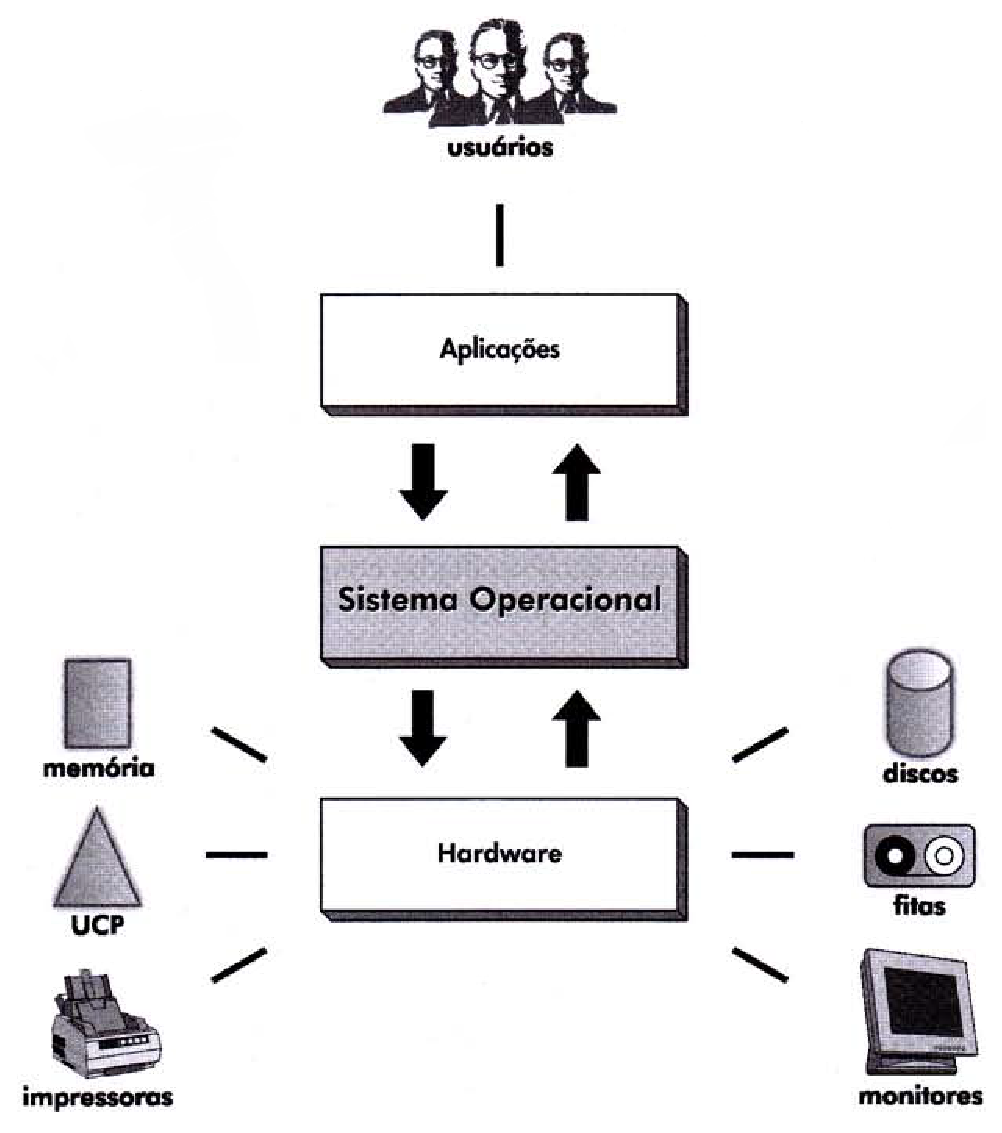
\includegraphics[keepaspectratio=true,scale=0.5]{figuras/so.eps}
	\fonte{\cite[p.~4]{machadomaia}.} % Referencia errada
\end{figure}

Analisando-se a definição proposta por \cite{limaevilaca} no início do primeiro parágrafo desta seção, entende-se como conveniente o fato citado por \cite{machadomaia} em que o sistema operacional é tido como uma espécie de interface entre o usuário e os recursos disponíveis no sistema computacional responsável por tornar esta comunicação transparente.

Como apresentado anteriormente, um sistema \texttt{RTOS} é um sistema operacional que proporciona um comportamento temporal previsível. Dessa forma idealmente um \texttt{RTOS} garante que a grande maioria de suas tarefas serão executadas em um prazo de tempo constante, independentemente da carga de trabalho a qual a \texttt{CPU} estará exposta naquele memento. Sistemas operacionais tradicionais como \texttt{Windows 8.1} e \texttt{Linux} não apresentam essa característica (determinismo), ao contrário de um \texttt{RTOS}, apenas garantem que as tarefas serão executadas, porém, o tempo de execução não é preciso sendo muitas vezes referido como "tempo médio de execução". Um \texttt{RTOS} é um sistema dirigido a eventos de \texttt{I/O}. Em função disso, a priori é necessário a apresentação das principais técnicas utilizadas no processo de transferência de dados entre o processador e a memória principal antes de dar continuidade a uma discussão mais aprofundada a respeito de um sistema \texttt{RTOS}.

Existem alguns tipos de aplicação que por mais que necessitem das características fornecidas por um \texttt{RTOS}, nem sempre será necessário à sua utilização. Isso é possível por meio da utilização do conceito de interrupções.
 
Sistemas embarcados utilizados em microcontroladores não costumam utilizar nenhuma espécie de sistema operacional, toda a sua programação é desenvolvida utilizando-se o conceito de \textit{superloop} que consiste em um único laço que é executado de maneira sequencial. A execução do \textit{superloop} é realizada indefinidamente enquanto a placa permanecer energizada. Nesse tipo de abordagem, eventos críticos (leitura de um sensor por exemplo) são tratados através de interrupções de \textit{hardware} que são executadas em primeiro plano. As demais operações do laço principal são executadas em segundo plano. A partir do instante em que a CPU do microcontrolador recebe um sinal de interrupção, inicia-se a chamada rotina de tratamento de interrupção. Essa rotina é caracterizada pela troca de contexto em que, o contexto atual (valores de registradores, contador de programa, etc.) é salvo na memória \texttt{RAM} e o tratamento da interrupção (rotina de \textit{software} específica) é iniciada. Após o término do tratamento da rotina, os registradores são restaurados e o controle é transferido para a instrução seguinte ao ponto de interrupção da aplicação. No caso de sistemas de tempo real pode ser que algumas aplicações críticas não possam ser interrompidas durante a sua execução. Nesse contexto começa a surgir o conceito de prioridade de interrupções, que é mais conhecido como interrupções mascaráveis e não-mascaráveis.

Interrupções mascaráveis podem ser desabilitadas pelo processador, enquanto as não-mascaráveis não, ou seja, deverão ser sempre atendidas. Pode ser que outras interrupções surjam enquanto o processador está executando uma rotina de tratamento, nesse caso, tem-se o surgimento dos vetores de interrupção que são armazenados em uma tabela na memória principal.

Porém, a abordagem comumente utilizada na programação de microcontroladores seja por questões de projeto ou por inexperiência do programador é a chamada de \texttt{I/O} programada conhecida também como “espera ocupada”. A utilização de interrupções permite que o processador execute outras tarefas na ausência de um sinal de interrupção. É como se o processador fosse “avisado” pelo dispositivo (sensor) o instante em que o evento ocorre. Já na \texttt{I/O} programada, conforme apresenta \cite{stail} o processador fica responsável pelo controle direto da operação de \texttt{I/O}, incluindo a detecção do estado do dispositivo, o envio de comandos de leitura ou escrita e a transferência de dados. É de se esperar que haverá um grande desperdício de uso de \texttt{CPU} caso o módulo de \texttt{I/O} seja mais lento que ela (o que ocorre na maioria das vezes). Em outras palavras, essa técnica faz com que o processador fique checando constantemente o estado do módulo \texttt{I/O} a fim de verificar o seu estado. Além do desperdício de tempo de processamento, o uso de \texttt{I/O} programada pode gerar inconsistências na detecção de eventos em códigos mais extensos; como o código é executado de maneira sequencial pode ser que, no instante de ativação de um sensor por exemplo, a execução esteja em um ponto em que isso não é tratado. Isso é muito comum em sistemas de monitoramento que são sistemas que podem ter que lidar com um grande número de sensores. 

Tanto no caso do uso de interrupções como na “espera ocupada” a \texttt{CPU} sempre é a responsável por intermediar a comunicação entre o módulo \texttt{I/O} e à memória principal. Existe uma técnica alternativa conhecida como \texttt{DMA (Direct Memory Access)} em que a transferência entre o módulo de \texttt{I/O} e a memória principal é feita diretamente sem a intervenção do processador.  Ainda segundo \cite{stail}, as duas primeiras formas de \texttt{I/O} apresentadas anteriormente possuem duas desvantagens inerentes: 

\begin{itemize}

	\item Taxa de transferência limitada pela velocidade com que o processador pode testar e servir um dispositivo;
	\item Ocupação do processador no gerenciamento da transferência, tendo que executar várias instruções a cada transferência. 

\end{itemize}

A grande sacada da técnica \texttt{DMA} consiste na presença de um módulo \texttt{DMA} capaz de simular o trabalho executado pelo processador, ou seja, tal módulo fica responsável por todo o gerenciamento da operação de entrada e saída entre o dispositivo e a memória principal. A utilização do barramento pelo módulo \texttt{DMA} pode ser realizado por meio de duas maneiras diferentes: o módulo força a \texttt{CPU} a liberar o barramento ou o usa quando a \texttt{CPU} não está o ocupando. A \autoref{tecnicaio} apresenta as características de cada uma das três técnicas de comunicação discutidas.

\begin{figure}[h]
	\centering
	\caption{\label{tecnicaio}Técnicas de \texttt{I/O}.}
		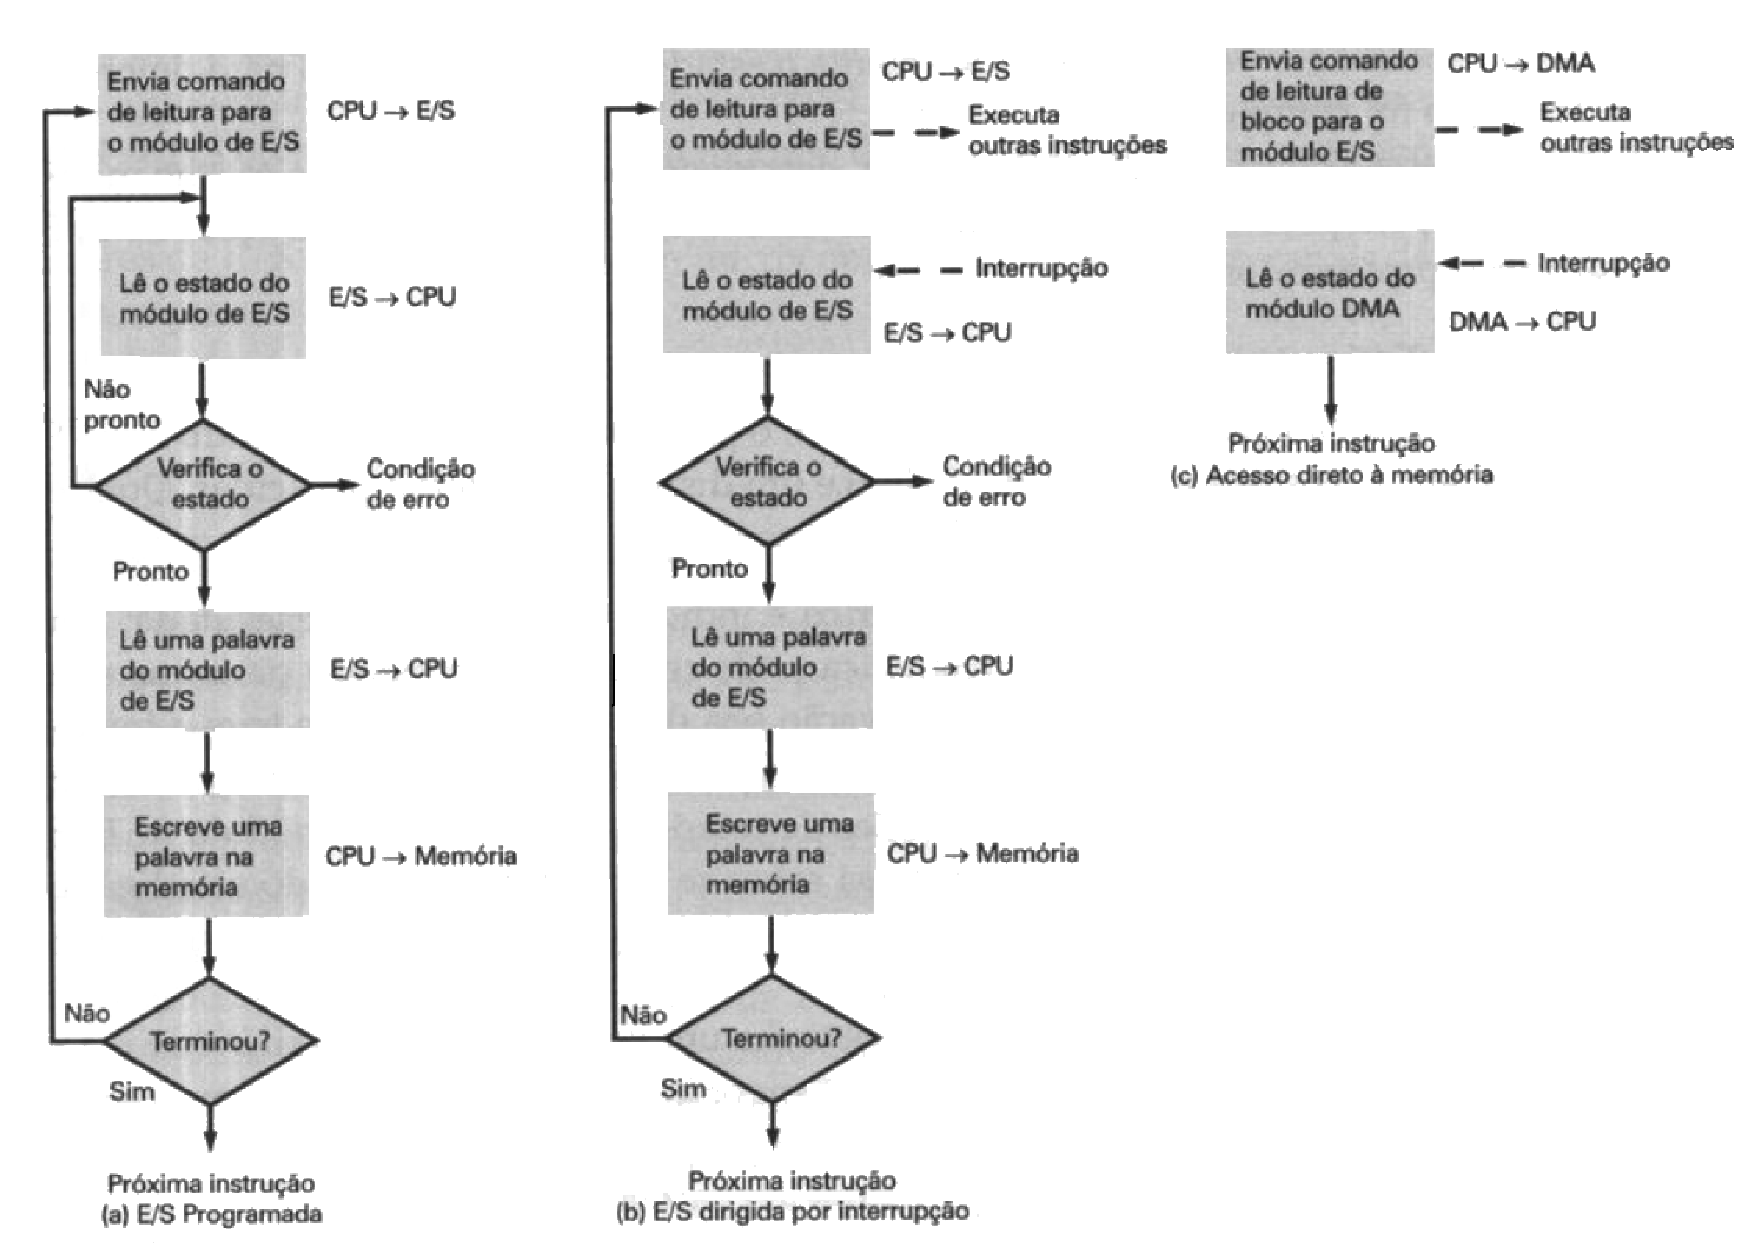
\includegraphics[keepaspectratio=true,scale=0.5]{figuras/tec.eps}
	\fonte{\cite[p.~4]{machadomaia}.} % Referencia errada
\end{figure}

Apesar das grandes vantagens associadas ao uso da técnica \texttt{DMA}, apenas microcontroladores mais robustos (destinados ao tratamento de arquivos de áudio \texttt{MP3}, \textit{streaming} de vídeo, etc.) possuem suporte a tal tecnologia. Entre os modelos de aplicação geral que possuem um módulo \texttt{DMA} estão a família de \texttt{chips AVR XMEGA} da \texttt{Atmel} e \texttt{PIC32} do \texttt{microchip}, além da plataforma \texttt{Arduino DUE} equipada com \texttt{chip ARM}.

A estratégia de utilização de interrupções sem a utilização de um \texttt{SO} é eficaz até certo ponto. A medida que o número de interrupções cresce o código tende a se tornar mais complexo e ineficiente em função do crescimento do vetor de interrupções\footnote{Tabela de endereços de memória que apontam para as rotinas de tratamento de interrupção.}. Nesse cenário pode ocorrer situações indesejáveis como estouro da pilha de execução, monopólio da \texttt{CPU} por um processo, entre outras.  Dessa forma é fácil perceber que, independentemente da técnica de \texttt{I/O} utiliza pelo programador, sem a utilização de um sistema operacional fica a seu cargo realizar todo o gerenciamento dos recursos. Esse gerenciamento envolve o controle de: memória e processos. O gerenciamento dessas duas entidades é algo complexo de se implementar (principalmente no que diz respeito ao gerenciamento de memória). Mais detalhes a respeito do gerenciamento de memória e de processos são discutidos na seção próxima seção.

Sistemas operacionais como um todo apresentam a grande vantagem de serem transparentes ao usuário no que diz respeito a gerencia de processos e memória de maneira bem mais eficiente e segura. No caso dos microcontroladores equipados com um \texttt{RTOS} temos além disso, a capacidade de transformar o conceito de \textit{superloop} em uma aplicação baseada em múltiplas tarefas que são adequadamente gerenciadas pelo \texttt{kernel} do sistema. 

\section{Gerenciamento de memória e escalonamento de processos} 

Nesta seção são apresentadas as principais atribuições de um sistema operacional que a grosso modo se resumem ao gerenciamento de memória e o escalonamento de processos.

\subsection{Escalonamento de processos} 

O gerenciamento da \texttt{CPU} consiste em uma das atividades mais importantes envolvidas em um sistema de computação. Deve-se ter políticas apropriadas responsáveis por determinar qual processo será o escolhido para fazer o uso da unidade central de processamento. Tais políticas são conhecidas como políticas de escalonamento. A parte do \texttt{SO} responsável por implementar os critérios da política de escalonamento é conhecida como escalonador. Independentemente da política a ser utilizada durante o escalonamento de processos é objetivo geral do escalonador manter a \texttt{CPU} a maior parte do tempo ocupada e balancear o seu uso entre os processos de acordo com a sua prioridade. Além disso, conforme apresenta \cite{machadomaia} existem alguns critérios que devem ser levados em conta em qualquer política de escalonamento, são eles:

\begin{itemize}

	\item Utilização do processador: Garante que o processador irá permanecer ocupado na maior parte do tempo;
	\item \texttt{Throughput}: Representa o número de processos executados em um determinado intervalo de tempo. Quanto maior o \texttt{throughput}, maior o número de tarefas executas em função do tempo. A maximização do \texttt{throughput} é desejada na maioria dos sistemas;
	\item Tempo de Processador: Se refere ao tempo que um processo leva no estado de execução durante seu processamento. As políticas de escalonamento não influenciam o tempo de um processo, sendo este tempo função apenas do código da aplicação e da entrada de dados;
	\item Tempo de Espera: Se refere ao tempo total que um processo permanece na fila de pronto durante seu processamento, aguardando para ser executado. A redução de tempo de espera dos processos é desejada pela maioria das políticas de escalonamento; 
	\item Tempo de Resposta: Se refere ao tempo decorrido entre uma requisição ao sistema ou à aplicação e o instante em que a resposta é exibida. Em geral, o tempo de resposta não é limitado pela capacidade de processamento do sistema computacional, mas pela velocidade dos dispositivos de \texttt{I/O}. 

\end{itemize}

Em linhas gerais \cite{machadomaia} afirmam que, “qualquer política de escalonamento busca otimizar a utilização do processador e o \texttt{throughput}, enquanto tenta diminuir os tempos de \texttt{turnaround}, espera e resposta”. 

São várias as técnicas utilizadas na operação de escalonamento de processos, algumas mais sofisticadas, outras nem tanto. O mesmo pode-se dizer em relação ao quesito complexidade, alguns algoritmos são mais eficientes, porém, complexos e vice e versa. O fato é que, não existe nenhuma solução ideal e que seja a prova de falhas. Os algoritmos escalonadores se dividem em dois grandes grupos, os preemptivos e os não preemptivos. O primeiro caso consiste nos algoritmos que permitem que um processo seja interrompido (por meio de um sinal de interrupção) durante a sua execução. Essa abordagem dá ao sistema a possibilidade de priorizar a execução de processos, como ocorre no caso de aplicações de tempo real. O último caso é basicamente o contrário do primeiro, como o próprio nome indica, ou seja, não existe a possibilidade de nenhum evento externo interromper a execução do processo que está fazendo uso da \texttt{CPU} no memento. As únicas possibilidades de o processo sair do estado de execução são: caso termine seu processamento ou execute uma instrução própria que faça isso.  Algoritmos não preemptivos não são condizentes com as propostas de um \texttt{RTOS} ou de qualquer sistema em que múltiplos processos requerem a sua atenção. A seguir são apresentados resumidamente alguns algoritmos populares que podem ser utilizados na implementação do escalonador. A descrição de cada técnica foi adaptada \cite[p.~137-150]{machadomaia}.

\begin{itemize}

	\item Escalonamento \texttt{First-In-First-Out (FIFO)}:
Nessa técnica, o processo que chegar primeiro ao estado de pronto é o selecionado para execução. Sua implementação exige apenas a criação de uma fila na qual os processos em estado pronto entrem no seu final e são escalonados quando chegam ao seu início. Quando o processo em execução termina seu processamento ou vai para o estado de espera, o primeiro processo da fila de pronto é escalonado. Apesar de simples, essa técnica apresenta um grave problema que consiste na impossibilidade de se prever quando um processo terá a sua execução iniciada. Além disso vale ressaltar que é um algoritmo não preemptivo;
	\item Escalonamento \texttt{Shortest-Job-First (SJF)}:
O algoritmo seleciona o processo em estado de pronto que necessitar de menos tempo de \texttt{CPU}. Como não é possível precisar previamente o tempo de processador para cada processo, uma estimativa é realizada utilizando-se análises estatísticas de execuções passadas dos programas. Caso o tempo informado ao \texttt{SO} for muito inferior ao tempo real, o sistema poderá interromper a execução do processo. O principal problema nesta implementação é a impossibilidade de estimar o tempo de processador para processos interativos, devido à entrada de dados ser uma ação imprevisível;
	\item Escalonamento Cooperativo:
Busca aumentar o grau de multiprogramação em políticas de escalonamentos que não possuam mecanismos de preempção, como o \texttt{FIFO} e o \texttt{SJF} não-preemptivo. Neste caso, um processo em execução pode voluntariamente liberar o processador retornando a fila de pronto. Sua principal característica está no fato de a liberação do processador ser uma tarefa realizada exclusivamente pelo processo em execução, ficando a seu cargo a verificação periódica de uma fila de mensagens para determinar se existem outros processos na fila de pronto. No caso de um processo não verificar a fila de mensagens, os demais não terão chance de serem executados até a liberação do processador pelo processo em execução;
	\item Escalonamento Circular:
É um escalonamento do tipo preemptivo, projetado especialmente para sistemas de tempo compartilhado. É muito semelhante ao \texttt{FIFO}, porém, quando um processo passa para o estado de execução, existe um tempo limite para o uso contínuo do processador denominado fatia de tempo ou quantum. O algoritmo concede uma nova fatia de tempo para cada processo toda vez que ele é escalonado para execução. A \autoref{circular} ilustra o funcionamento do algoritmo. O valor da fatia de tempo varia de acordo da arquitetura de cada sistema operacional e este valor está diretamente relacionado ao desempenho da política de escalonamento circular. No caso em que a fatia de tempo tenha um valor muito alto, o escalonamento circula irá apresentar o mesmo comportamento do escalonamento \texttt{FIFO}. Sua principal vantagem é a não permissão da monopolização da \texttt{CPU} por um processo, já que a sua fatia de tempo é definida pelo sistema. Por outro lado, processos do tipo \texttt{CPU-bound} são beneficiados no uso do processador em relação a processos \texttt{I/O-bound} ocasionando um balanceamento desigual do processador entre os processos;

\begin{figure}[h]
	\centering
	\caption{\label{circular}Escalonamento circular.}
		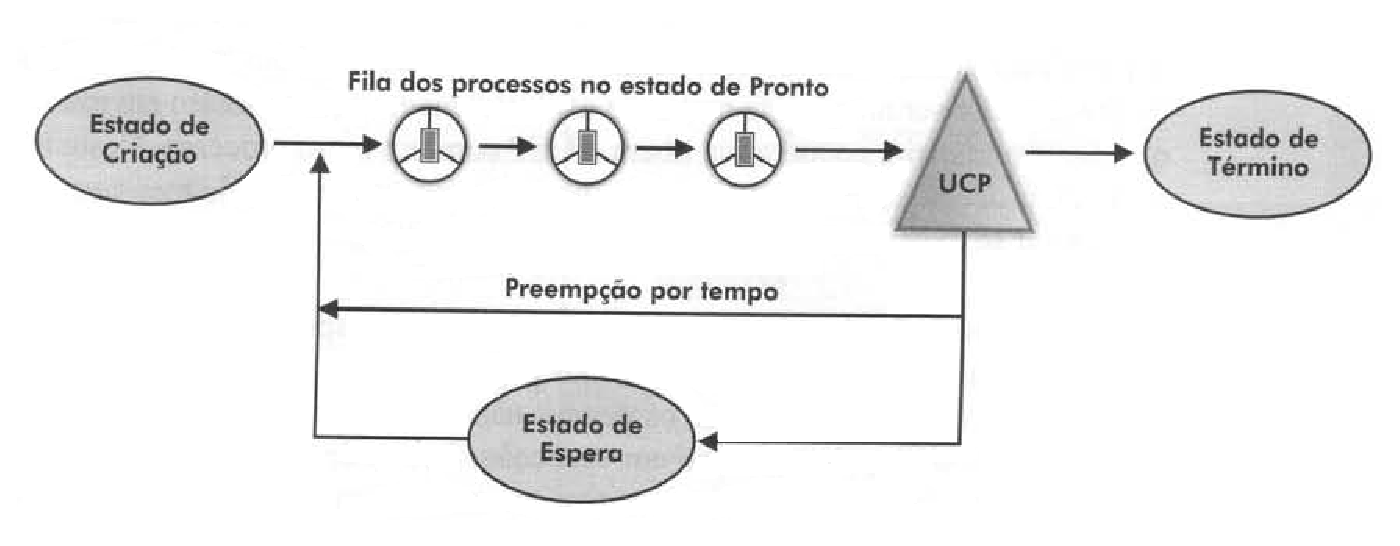
\includegraphics[keepaspectratio=true,scale=0.5]{figuras/circular.eps}
	\fonte{\cite[p.~142]{machadomaia}.} % Referencia errada
\end{figure}

	\item Escalonamento por Prioridades:
É um escalonamento preemptivo realizado com base em um valor associado a prioridade de execução de cada processo. Processos com maiores prioridades são sempre os primeiros a serem escolhidos para execução, processos com prioridades iguais são escolhidos de acordo com o critério \texttt{FIFO}. Como não existe o conceito de fatia de tempo, um processo em execução não pode sofrer preempção por tempo. Dessa forma a perda do uso do processador só ocorrerá no caso de uma mudança voluntária para o estado de espera ou quando o processo passa para o estado de pronto. A implementação dessa lógica é realizada através de uma interrupção de \textit{clock}, sendo que, no caso do surgimento de um processo de maior prioridade na fila de pronto, o \texttt{SO} realiza a preempção. Esse tipo de escalonamento também pode ser alternativamente implementado de maneira não-preemptiva, neste caso um processo não perderá o uso de \texttt{CPU} mesmo que um de maior prioridade surja na fila de prontos (o processo será apenas alocado para o início da fila). Os valores de prioridades constituem uma característica de \textit{software} e podem ser fixos ou dinâmicos. Um dos principais problemas no escalonamento por prioridades é o \texttt{starvation}. Processos de baixa prioridade podem não ser escalonados, permanecendo indefinidamente na fila de pronto. Isso pode ser resolvido por meio da aplicação da técnica conhecida como \texttt{aging}, que consiste em incrementar gradualmente a prioridade de processos que permanecem por muito tempo na fila de pronto;
	\item Escalonamento Circular com Prioridades:
Neste tipo de escalonamento existe o conceito de fatia de tempo aliada ao conceito de prioridade. Um processo permanece em execução até que termine seu processamento, ou sofra uma preempção por tempo. A \autoref{circularpri} ilustra o seu funcionamento. Sua principal vantagem é permitir o melhor balanceamento no uso da \texttt{CPU}, com a possibilidade de diferenciar o grau de importância dos processos;

\begin{figure}[h]
	\centering
	\caption{\label{circularpri}Escalonamento circular com prioridades.}
		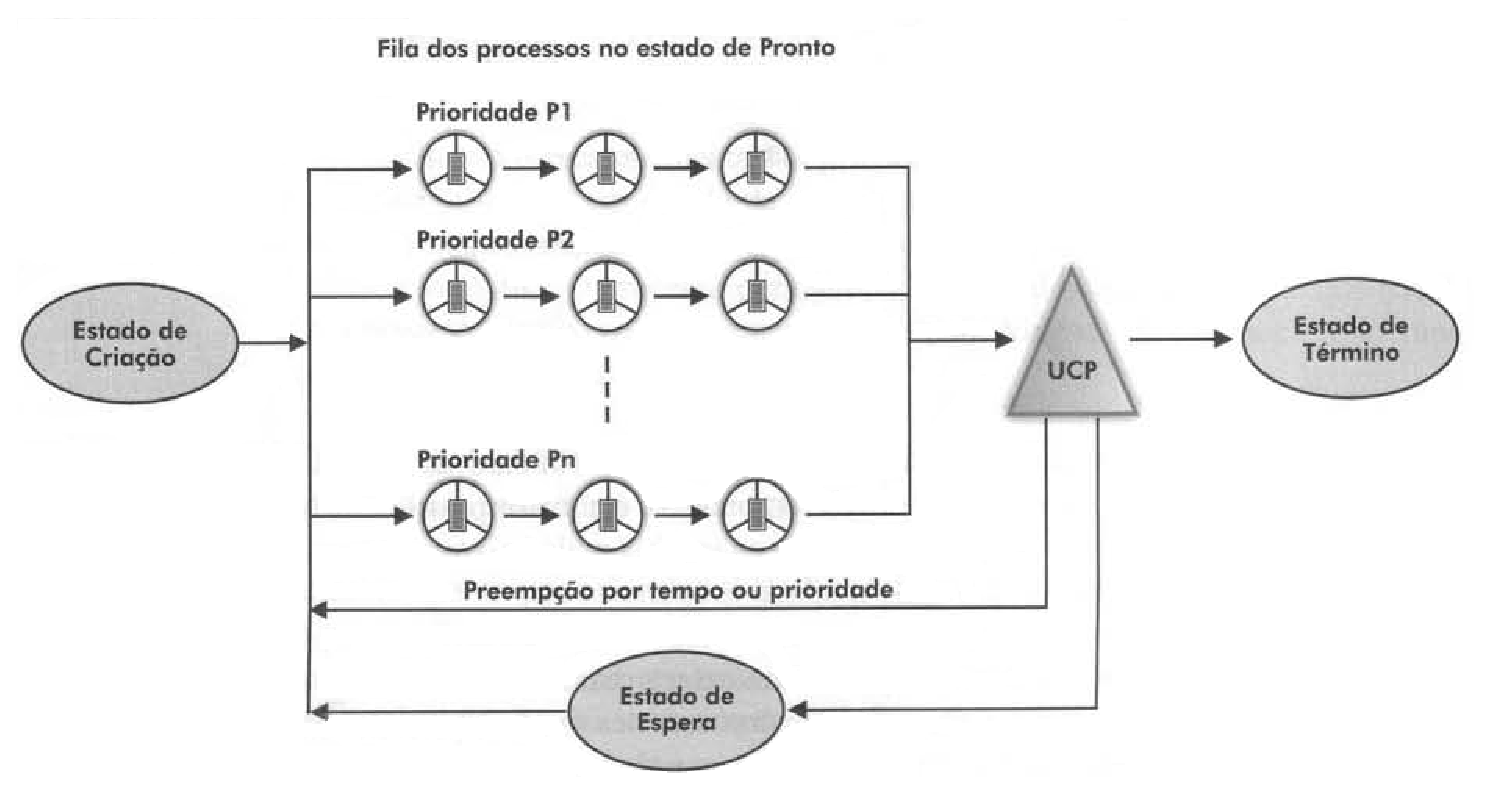
\includegraphics[keepaspectratio=true,scale=0.5]{figuras/circularpri.eps}
	\fonte{\cite[p.~146]{machadomaia}.} % Referencia errada
\end{figure}

	\item Escalonamento por Múltiplas Filas:
Nesta metodologia existem diversas filas de processos no estado de pronto, cada qual com uma prioridade específica. Cada fila tem características próprias, como importância para a aplicação, tipo de processamento ou área de memória necessária. Em função de cada processo possuir características distintas, torna-se difícil que um único mecanismo de escalonamento seja adequado a todos. Aí que reside a principal vantagem do escalonamento por múltiplas filas já que é possível a convivência de escalonamento distintos (\texttt{FIFO} ou circular) em cada fila em um mesmo \texttt{SO}. Não existe prioridade, isso se torna uma característica associada à fila. O processo em execução sofre preempção caso outro processo entre em uma fila de maior prioridade. O \texttt{SO} só poderá escalonar um processo de determinada fila caso todas as filas de maior prioridade estejam vazias. A \autoref{multiplas} ilustra a técnica de escalonamento por múltiplas filas;
	\item Escalonamento por Múltiplas Filas com Realimentação:
É semelhante ao escalonamento por múltiplas filas, porém os processos podem trocar de fila durante seu processamento. A vantagem disso é que o SO pode identificar dinamicamente o comportamento de cada processo, direcionando-o para a fila com prioridade de execução e mecanismo de escalonamento mais adequados ao longo do seu processamento. Um mecanismo FIFO adaptado com fatia de tempo é implementado para o escalonamento em todas as filas, com exceção da fila de menor prioridade que continua utilizando o escalonador circular. A fatia de tempo destinada a cada processo varia de acordo com a sua prioridade. Este tipo de escalonamento atende as necessidades dos diversos tipos de processos. No caso de processos I/O-bound, um tempo de resposta adequado é obtido, já que esses processos têm prioridades mais altas por permanecerem a maior parte do tempo nas filas de maior prioridade, em que dificilmente sofrerão preempção por tempo. 

\end{itemize}

\begin{figure}[h]
	\centering
	\caption{\label{multiplas}Escalonamento por múltiplas filas.}
		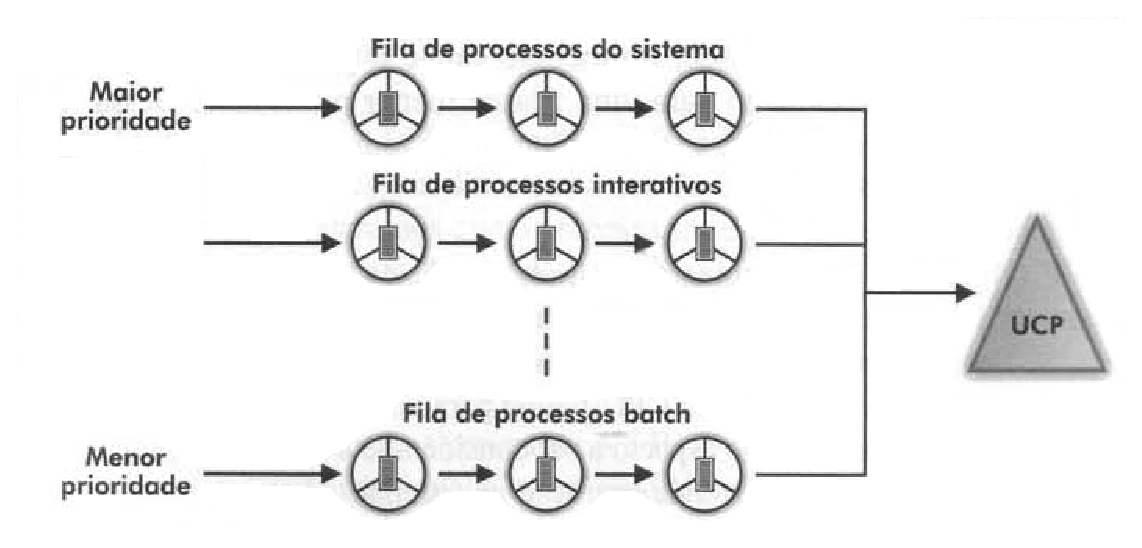
\includegraphics[keepaspectratio=true,scale=0.5]{figuras/multiplas.eps}
	\fonte{\cite[p.~147]{machadomaia}.} % Referencia errada
\end{figure}

Em linhas gerais vale a pena destacar que sistemas com prioridade dinâmica são mais complexos de serem implementados, porém, apresentam um menor tempo de resposta. Segundo \cite{machadomaia} atualmente a maioria dos \texttt{SOs} de tempo compartilhado utiliza o escalonamento circular com prioridades dinâmicas. No caso de sistemas de tempo real, a metodologia mais indicada é a pôr prioridades. Nesse tipo de sistema não deverá haver o conceito de fatia de tempo e a prioridade de cada processo deverá ser estática. 

\subsection{Gerenciamento de memória}

Em sistemas multiprogramados a memória é dividida basicamente em duas partes, a memória de usuário e a memória do sistema. A área de memória do usuário é subdividida de maneira que acomode vários processos. Essa subdivisão é feita pelo \texttt{SO} e ocorre dinamicamente, sendo tal procedimento conhecido como gerenciamento de memória. Assim como no gerenciamento de processos, o gerenciamento de memória é vital para um sistema multiprogramado. Deve-se alocar a memória de maneira eficiente e com a maior quantidade possível de processos.  Os primeiros sistemas operacionais utilizavam técnicas de particionamento estáticas em que, o tamanho de cada partição é fixo. O controle é realizado por meio de uma tabela que contém o endereço inicial e final de cada partição, além do seu tamanho e se a mesma está ou não em uso. Quando um programa precisa ser carregado na memória, o \texttt{SO} realiza uma busca na tabela a fim de encontrar uma partição livre onde o programa possa ser carregado. O grande problema da alocação fixa é o surgimento do fenômeno conhecido como fragmentação interna de memória. Isso ocorre porque nem sempre os programas preenchem totalmente as partições onde são carregados. A \autoref{particao} apresenta a estrutura de uma tabela de partições. Para solucionar-se o problema da segmentação interna foi criado um método de alocação dinâmica em que o conceito de partições fixas foi eliminado. Cada programa utiliza apenas o espaço que necessita, o problema da fragmentação interna é resolvido. Porém, a partição dinâmica produz um novo tipo de segmentação, conhecida como segmentação externa.

\begin{figure}[h]
	\centering
	\caption{\label{particao}Tabela de alocação de partições.}
		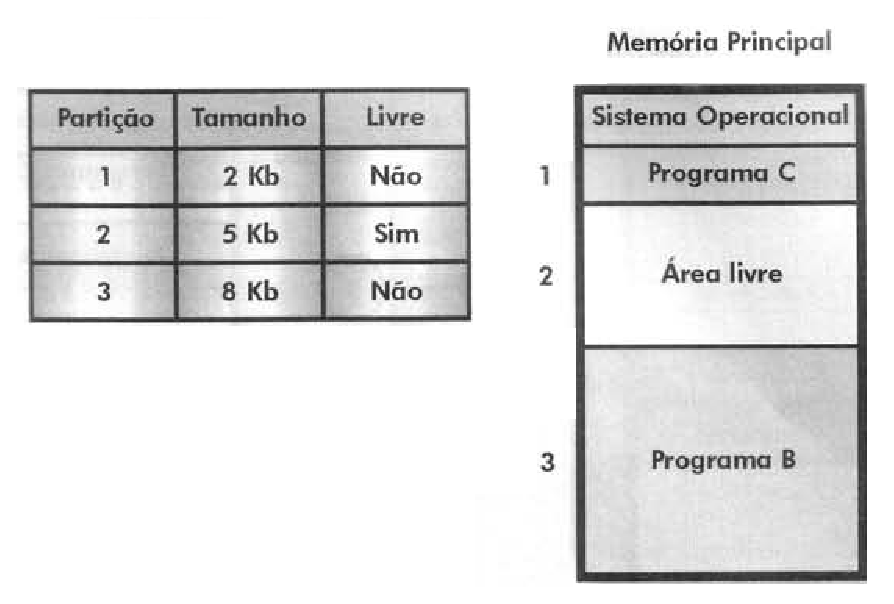
\includegraphics[keepaspectratio=true,scale=0.5]{figuras/particao.eps}
	\fonte{\cite[p.~161]{machadomaia}.} % Referencia errada
\end{figure}

Isso ocorre na medida em que a memória é utilizada e a entrada e saída de processos vai produzindo espaços vazios cada vez menores ao longo do espaço de endereçamento. Nesse contexto a memória poderá até ter o espaço suficientemente livre para que um determinado processo seja alocado, entretanto, geralmente tal espaço não está disposto de maneira contínua o que impede a sua alocação. A tendência é que com o passar do tempo a memória se torne cada vez mais fragmentada e a sua utilização diminua. Existe uma técnica apresentada por \cite{stail} que acaba em parte com esse problema; denominada compactação consiste em uma varredura que é executada de tempos em tempos pelo \texttt{SO} com o objetivo de trocar os processos de lugar, agrupando dessa forma todas as áreas livres de memória. A desvantagem é que esse processo consome tempo útil de processamento. 
Conforme apresenta \cite{machadomaia}, existem basicamente três estratégias de alocação de espaços na memória principal, são elas:

\begin{itemize}

	\item \texttt{Best-fit}:
Essa técnica visa escolher a melhor partição, ou seja, a que o programa deixa o menor espaço sem utilização. Entretanto, a sua grande desvantagem é a sua tendência de fazer com que a memória fique cada vez mais com áreas não-contíguas, aumentando o problema da fragmentação;
	\item \texttt{Worst-fit}:
O conceito dessa técnica é o inverso da anterior, ou seja, é escolhida a partição que deixa o maior espaço sem utilização. Isso é interessante pois maiores partições surgirão o que permite um número maior de programas utilizando a memória, amenizando o problema da fragmentação;
	\item \texttt{First-fit}:
É escolhida a primeira partição livre de tamanho suficiente para carregar o programa. A lista de áreas livres é ordenada de maneira crescente por endereços. Em função de utilizar as áreas livres de endereços mais baixos, existe uma grande chance de se obter uma grande partição livre nos endereços de memória mais altos. É a estratégia mais rápida, consumindo menos recursos do sistema.

\end{itemize}

\section{Redes de comunicação - Implementação e protocolos de funcionamento} 

A comunicação entre o microcontrolador e o servidor \textit{Web} será realizada de acordo 
com os padrões da comunicação cliente-servidor, onde o microcontrolador fará o papel 
de cliente e a interface \textit{Web} juntamente com o banco de dados será o servidor. A comunicação 
entre o cliente e o servidor será realizada através do protocolo \texttt{HTTP (HyperText Transfer Protocol)} 
que faz parte da camada de aplicação da \textit{Web}. O programa inserido no microcontrolador conversará com 
o programa criado no servidor através da troca de mensagens \texttt{HTTP}.
O \texttt{HTTP} utiliza o \texttt{TCP} como protocolo de transmissão de dados, essa operação é
descrita por \cite[p.~73]{kurose2010} da seguinte forma:

\begin{citacao}
``O cliente \texttt{HTTP} primeiramente inicia uma conexão \texttt{TCP} com o servidor. Uma vez
estabelecida a conexão, os processos do browser e do servidor acessam o \texttt{TCP} por
meio de suas interfaces \textit{sockets}.
O cliente envia mensagens de requisição \texttt{HTTP} para sua interface \textit{socket} e recebe
mensagens de resposta \texttt{HTTP} de sua interface \textit{socket}. De maneira semelhante, o
servidor \texttt{HTTP} recebe mensagens de requisição de sua interface \textit{socket} e envia
mensagens de resposta para sua interface \textit{socket}. Assim o cliente envia uma
mensagem para sua interface \textit{socket}, a mensagem sai de suas mãos e “passa para as
mãos do \texttt{TCP}” [...]. O \texttt{TCP} prove ao \texttt{HTTP} um serviço confiável de transferência de
dados, o que implica que toda mensagem de requisição \texttt{HTTP} emitida por um
processo cliente chegara intacta ao servidor. De maneira semelhante, toda mensagem
de resposta \texttt{HTTP} emitida pelo processo servidor chegará intacta ao cliente [...].``
\end{citacao}

\begin{figure}[h]
	\centering
	\caption{\label{fig5}Processos de aplicação, \textit{sockets} e protocolos de transporte subjacente.}
		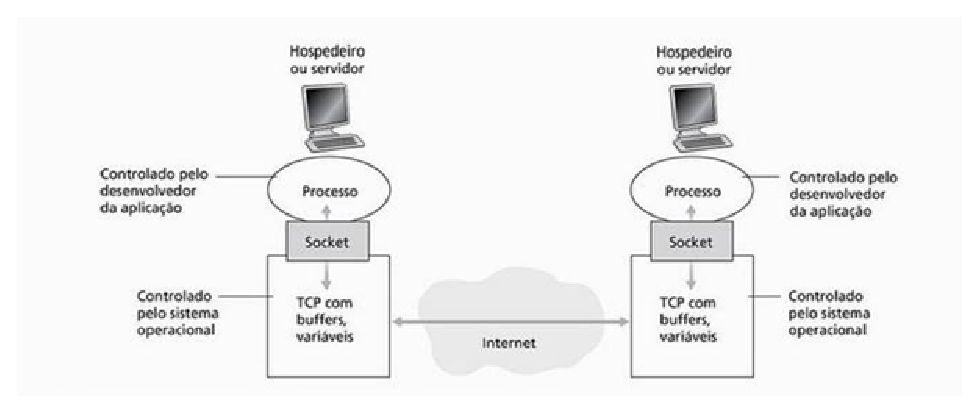
\includegraphics[keepaspectratio=true,scale=1]{figuras/socket.eps}
	\fonte{\cite[p.~66]{kurose2010}.} % Referencia errada
\end{figure}

Existem dois tipos de mensagens \texttt{HTTP} conforme explicado por \cite[p.~76]{kurose2010},
as mensagens de requisição e as mensagens de resposta. As mensagens de requisição possuem
um cabeçalho com as informações da mensagem. Uma linha deste cabeçalho diz respeito ao
método que a mensagem de requisição carrega. Os métodos existentes são \textit{GET}, \textit{POST} e
\textit{HEAD}. O método \textit{GET} é normalmente o mais utilizado, ele consiste na requisição de um objeto
feita a um servidor. O método \textit{HEAD} é semelhante ao \textit{GET}, porém este método não será
abordado neste projeto. O método \textit{POST} é utilizado, por exemplo, quando um usuário preenche
um formulário e envia as alterações para o servidor. Segundo descreve \cite[p.~77]{kurose2010}:

\begin{citacao}
''Com uma mensagem \textit{POST}, o usuário continua solicitando uma página \textit{Web} ao
servidor, mas o conteúdo específico dela depende do que o usuário escreveu nos
campos do formulário. Se o valor do campo de método for \textit{POST}, então o corpo de
entidade conterá o que o usuário digitou nos campos do formulário.``
\end{citacao}

A mensagem de resposta é utilizada quando o servidor envia uma mensagem para o
cliente com o intuito de responder a uma mensagem de requisição.

\begin{figure}[h]
	\centering
	\caption{\label{req-resp}Comportamento de requisição-resposta do \texttt{HTTP}.}
		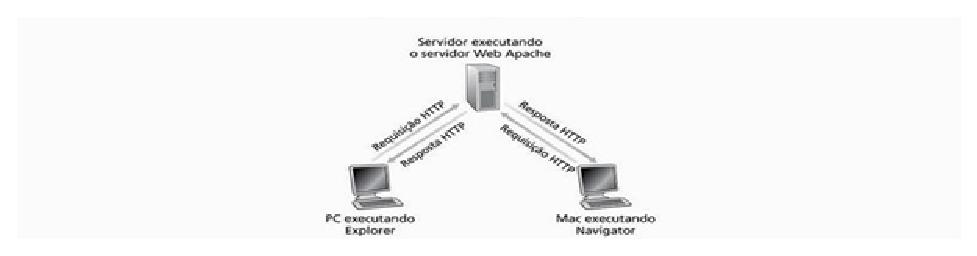
\includegraphics[keepaspectratio=true,scale=1]{figuras/req-resp.eps}
	\fonte{\cite[p.~73]{kurose2010}.} % Referencia errada
\end{figure}


O formato das mensagens de requisição é apresentado na \autoref{requisicao}.

\begin{figure}[h]
	\centering
	\caption{\label{requisicao}Cabeçalho de uma mensagem de requisição \texttt{HTTP}.}
		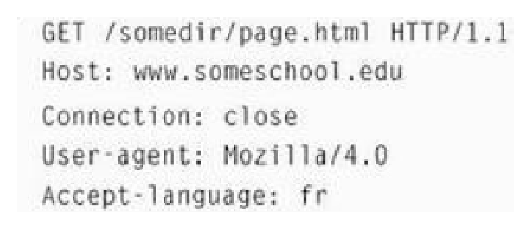
\includegraphics[keepaspectratio=true,scale=1]{figuras/requisicao.eps}
	\fonte{\cite[p.~76]{kurose2010}.} % Referencia errada
\end{figure}

O significado de cada linha é apresentado por \cite[p.~76]{kurose2010}. A primeira linha é composta 
pelo método utilizado de conexão, o endereço da requisição ou destino da mensagem e a 
versão do \texttt{HTTP}. A segunda linha apresenta o endereço de onde foi feita a requisição, 
ou seja, a origem. Na terceira linha o campo \textit{“Connection”}  representa o tipo de conexão 
utilizado. Os tipos de conexões existentes são classificados como persistentes ou não 
persistentes. Em conexões persistentes o cliente estabelece uma conexão com o servidor 
permanecendo, conectado enquanto houver a transferência de dados ou o cliente desejar. 
Já em conexões não persistentes, os clientes e servidores estabelecem uma conexão apenas 
pelo período necessário ao envio de uma mensagem. Neste caso o campo \textit{“Connection: Close”} 
estabelece uma conexão não persistente, onde o cliente fica conectado ao servidor somente 
até a resposta da mensagem de requisição. A quarta linha apresenta o tipo do \textit{browser} que 
está fazendo a requisição ao servidor. A quinta linha especifica a preferência de linguagem 
que o cliente deseja receber os dados, caso a linguagem desejada não esteja disponível a mensagem de resposta 
conterá a linguagem padrão do servidor.

Já a mensagem de resposta é apresentada na \autoref{resposta}.

\begin{figure}[h]
	\centering
	\caption{\label{resposta}Cabeçalho de uma mensagem de resposta \texttt{HTTP}.}
		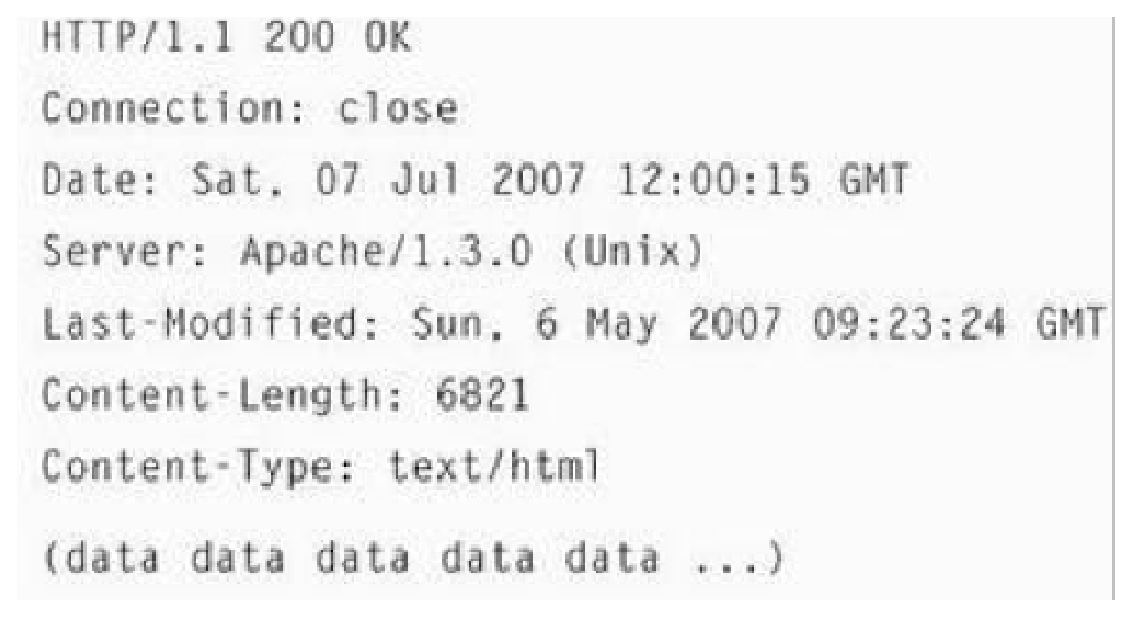
\includegraphics[keepaspectratio=true,scale=0.6]{figuras/resposta.eps}
	\fonte{\cite[p.~78]{kurose2010}.} % Referencia errada
\end{figure}

Conforme apresenta \cite[p.~78]{kurose2010}, a mensagem de resposta é dividida em três seções.
Uma linha inicial ou de estado, seis linhas de cabeçalho e em seguida o corpo da mensagem.
A primeira linha mostra a versão do \texttt{HTTP} seguido da confirmação de encontro do objeto requisitado.
Na segunda linha é estabelecido se a conexão é persistente ou não. A terceira linha indica a data 
e hora em que o servidor enviou a mensagem de resposta. A quarta linha indica a versão de 
\textit{software} que o servidor está utilizando, de forma análoga, esse campo é semelhante ao campo 
\textit{“User-agent”} indicado na mensagem de requisição. A quinta linha indica a data e hora em que 
o objeto requisitado foi criado ou modificado pela última vez. Na sexta linha é apresentado 
o tamanho em \textit{bytes} do objeto que está sendo enviado. A sétima linha mostra o formato do objeto 
a ser enviado. Por fim é apresentado o conteúdo de dados requisitado pelo cliente.

Considerando o projeto a ser desenvolvido os funcionários da empresa ou administradores 
farão papel de clientes no processo de gerenciamento. Eles irão fazer requisições de dados
ao servidor e utilizar esses dados requisitados para otimizar o gerenciamento da empresa. 
Ao requisitar os dados do servidor os funcionários e/ou administradores estarão fazendo uso 
implícito do método \textit{GET}. Já do lado dos microcontroladores que também são clientes, o método 
utilizado na comunicação \texttt{HTTP} será o \textit{POST}, pois os microcontroladores apenas enviarão pulsos 
digitais ou informações que serão tratadas no servidor.

\section{A linguagem \textit{Java}}

A linguagem \texttt{Java} foi criada pela antiga \texttt{Sun Microsystems} com objetivo sendo direcionado ao consumidor 
de produtos e usuários leigos. Em 1992 a \texttt{Sun} criou um time para desenvolver inovações tecnológicas. 
Esse time foi liderado por \texttt{James Gosling}, considerado pai do \texttt{Java}. \texttt{James Gosling} e seu time tinham 
como objetivo o desenvolvimento de um interpretador para pequenos dispositivos eletrônicos. A ideia 
no princípio fracassou devido a divergência de ideias e elevados custos. Com o crescimento da \textit{Web} a 
\texttt{Suns} percebeu que poderia utilizar sua ideia para rodar pequenas aplicações dentro de um \texttt{browser}. Seu 
objetivo era que a linguagem \texttt{Java} rodasse nos diferentes tipos de \texttt{browser} e sistemas operacionais 
existentes na época. No ano de 2009, a \texttt{Oracle} comprou a \texttt{Sun} fortalecendo a marca. Desde então, a \texttt{Oracle} 
juntamente com a \texttt{IBM} foram as empresas que mais investiram na linguagem Java \cite{caelumjava}.

Para executar uma aplicação \texttt{Java} é necessário uma máquina virtual que interpreta e executa as operações
encapsuladas em \textit{bytecode} da linguagem. Essa máquina virtual recebe o nome de \texttt{JVM (Java Virtual Machine)}. 
Esta característica importante da linguagem \texttt{Java}, permite que uma aplicação \texttt{Java} possa ser executada em qualquer
sistema operacional, necessitando apenas da \texttt{JVM} \cite{caelumjava}.

\begin{figure}[h]
	\centering
	\caption{\label{virtual}Representação da tradução de \textit{bytecodes} para chamadas do sistema operacional.}
		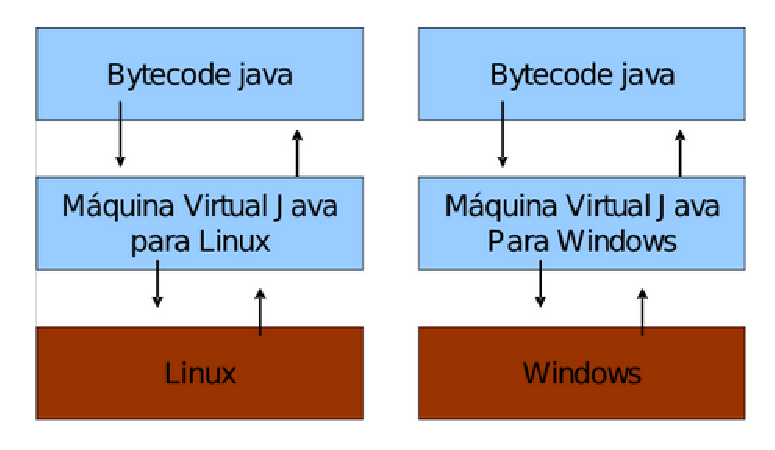
\includegraphics[keepaspectratio=true,scale=1]{figuras/virtual.eps}
	\fonte{\cite[p.~6]{caelumjava}.} % Referencia errada
\end{figure}

Para desenvolver uma aplicação \texttt{Java} é necessário a utilização do \texttt{JDK (Java Development Kit)}. 
O \texttt{JDK} é um pacote disponibilizado pela \texttt{Oracle} e é composto por um conjunto de utilitários necessários
para criação e execução de aplicações em \texttt{Java}. Neste pacote está incluso um outro pacote chamado de 
\texttt{JRE (Java Runtime Environment)}. O \texttt{JRE} é formado pela \texttt{JVM} e bibliotecas da linguagem.

\texttt{Java} é uma ferramenta poderosa para desenvolvimento de aplicações \textit{Web}. Tal tecnologia  possui 
um extenso conjunto de ferramentas e padronizações que são agrupadas em um pacote chamado de \texttt{Java Plataform}, 
que visam economizar tempo e dinheiro no ciclo de desenvolvimento. Foi escolhida 
a linguagem \texttt{Java} para o desenvolvimento da aplicação \textit{Web}, por ser uma linguagem orientada a objetos robusta de enorme 
versatilidade e importância no cenário atual da computação mundial.

Existe uma plataforma \texttt{Java} exclusiva para o desenvolvimento \textit{Web}. Esta plataforma é chamada de \texttt{Java EE 
(Java Plataform, Enterprise Edition)}. A plataforma \texttt{Java EE} possui bibliotecas e funcionalidades já criadas, 
baseadas em componentes modulares que são executados em servidores de aplicações. Esta plataforma é composta 
de uma série de tecnologias com objetivos distintos, as mais conhecidas são:

\begin{itemize}

	\item \texttt{Servlets}: São códigos escritos em \texttt{Java} e são executados no servidor para gerar conteúdo dinâmico para \textit{Web};
	\item \texttt{JSP (JavaServer Pages)}: É uma especialização de um \texttt{Servlet} também utilizada para gerar conteúdo dinâmico;
	\item \texttt{JSF (JavaServer Faces)}: É um \textit{framework Web} baseado em \texttt{Java}, foi criado com o intuito de facilitar a criação 
	de telas (interface) e aumentar a produtividade no desenvolvimento de sistemas \textit{Web};
	\item \texttt{JPA (Java Persistence API)}: É uma \texttt{API} padrão do \texttt{Java} utilizada para persistência dos dados onde são utilizados 
	conceitos de mapeamento objeto-relacional;
	\item \texttt{EJB (Enterprise Java Beans)}: São componentes que são executados no servidor com o objetivo de oferecer segurança 
	e facilidade na produção de sistemas \textit{Web}.

\end{itemize}

A aplicação \texttt{Java} \textit{Web} a ser criada terá como principal objetivo receber e tratar os dados dos eventos reportados pelos
serviços clientes, como o microcontrolador, conforme descreve \cite{marcilio2004}: 

\begin{citacao}
''Geralmente é bastante conveniente executar código de aplicação no servidor de
banco de dados, ao invés de simplesmente recuperar dados executar a lógica da
aplicação em processos separados. \textit{Stored Procedures} possibilitam que a lógica da
aplicação seja armazenada e executada no servidor.``
\end{citacao}

O desenvolvimento de \textit{softwares} que utilizam o conceito de programação orientada a objetos trouxe inúmeros benefícios 
aos desenvolvedores de \textit{software}, como o favorecimento do reuso ou extensão de classes criadas em outros projetos, 
conforme apresenta \cite[p.~1]{soares8}. Normalmente os sistemas \textit{Web} são distribuídos portanto, a orientação a objetos é um
importante paradigma nesse contexto, simplificando o acesso de diferentes usuários a quaisquer objetos.  
Em geral a programação orientada a objetos trouxe muitas facilidades no desenvolvimento de \textit{softwares}, mas como 
qualquer outro estilo de programação ela possui seus limites e não elimina alguns problemas. Parte desses problemas 
são destacados por \cite[p.~16]{antonio2005} como entrelaçamento, espalhamento, manutenibilidade e reusabilidade. Entretanto
é importante ressaltar que o entrelaçamento consiste no acréscimo demasiado de código.

\section{A linguagem \textit{HTML}}

A sigla \texttt{HTML} significa \texttt{HyperText Markup Language}, ou seja, linguagem de Marcação de Hipertexto. Consiste em uma linguagem 
de marcação utilizada para produção de páginas \textit{Web}. Foi criada por \texttt{Tim Barners} na década de 1990.

A linguagem \texttt{HTML} permite a criação de páginas na \textit{World Wide Web}, com imagens, textos, formulários, listas e conexões
em hipertexto a outras páginas e arquivos. Para se escrever em \texttt{HTML} pode-se utilizar um editor de texto especial para
linguagem ou um simples editor de texto, desde que sejam respeitados os comandos da linguagem. 
Os comandos \texttt{HTML} aparecem sempre na forma <comando>, escritos entre “<” e “>” para se diferenciarem do resto do texto 
em uma página. A \autoref{html} mostra um simples exemplo criado na linguagem \texttt{HTML}.

\begin{figure}[h]
	\centering
	\caption{\label{html}Estrutura de um código \texttt{HTML}.}
		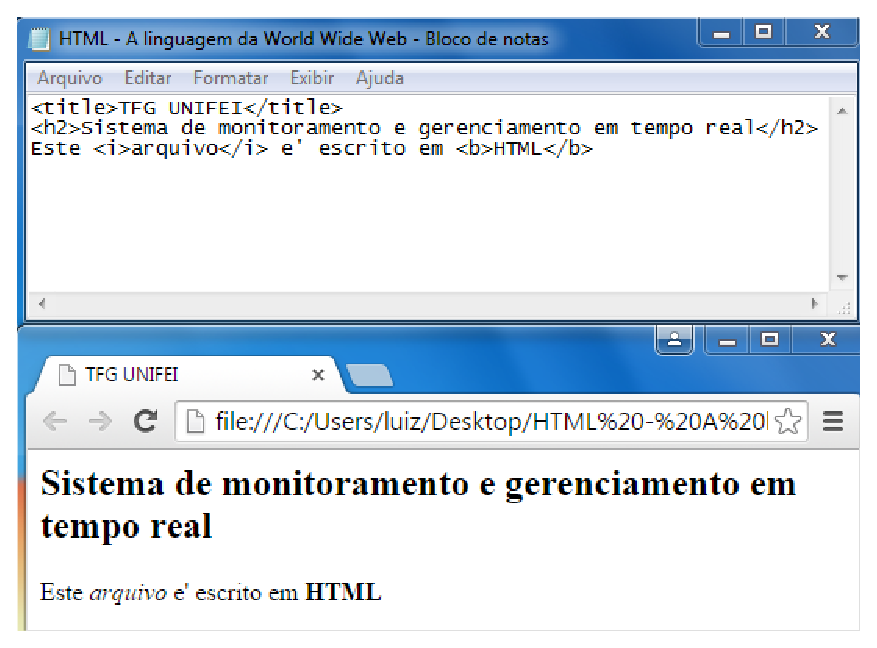
\includegraphics[keepaspectratio=true,scale=0.7]{figuras/html.eps}
	\fonte{Autoria própria.}
\end{figure}

\section{\textit{Servlets}}

No princípio do surgimento da \textit{Web} a maioria das páginas possuíam apenas conteúdos estáticos, compostos por códigos escritos
no formato \texttt{HTML}. Esses códigos eram responsáveis por apresentar em sua maior parte textos, imagens, animações e outros 
conteúdos de caráter estático. Com o passar do tempo surgiu a necessidade da criação de páginas de conteúdo dinâmico, baseadas
nas requisições em tempo real dos usuários. Em páginas com conteúdo dinâmico o usuário faz uma requisição ao servidor, que 
por sua vez processa essa requisição e retorna uma resposta. Na plataforma \texttt{Java} a principal tecnologia capaz de 
gerar páginas dinâmicas são as \texttt{Servlets} conforme apresenta \cite[p.~52]{caelumweb}.

O nome \texttt{Servlet} é derivado do conceito de pequeno servidor (“servidorzinho” em inglês). O seu principal papel é o de responder
a requisições \texttt{HTTP}. Em \texttt{Java}, um \texttt{Servlet} é representado como um objeto de uma classe \texttt{Java}. Os \texttt{Servlets} utilizam o mesmo modelo 
apresentado no protocolo \texttt{HTTP}. Este modelo é chamado de requisição/resposta. Cada \texttt{Servlet} é um objeto que possui como 
parâmetro dois campos: \textit{request} (requisição) e \textit{response} (resposta). Um \texttt{Servlet} pode responder a requisições dos mais diversos 
tipos de protocolo e não somente o \texttt{HTTP} \cite[p.~53]{caelumweb}. Neste trabalho será abordado apenas as requisições e repostas 
com o protocolo \texttt{HTTP} .

\begin{figure}[h]
	\centering
	\label{fig6}
	\caption{\label{httpgetpost}Métodos de um \texttt{Servlet HTTP}.}
		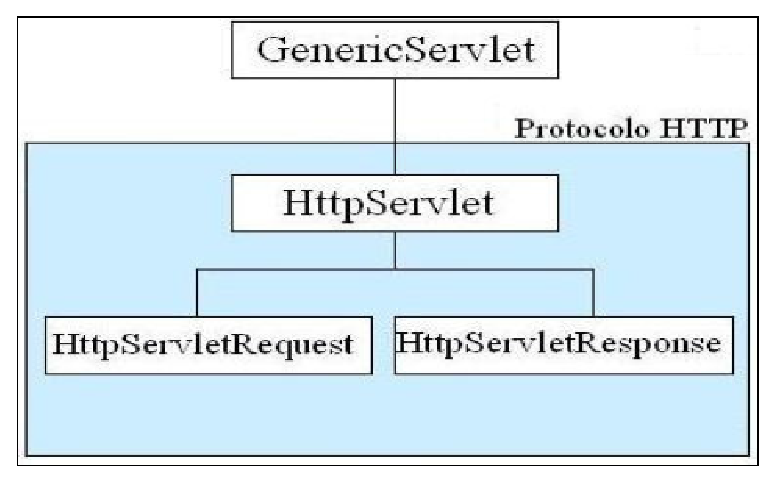
\includegraphics[keepaspectratio=true,scale=1]{figuras/httpgetpost.eps}
	\fonte{\cite[p.~18]{barale}.} 
\end{figure}

A classe que possui as bibliotecas necessárias a implementação de um \texttt{Servlet} para o protocolo \texttt{HTTP} é chamada de \texttt{HTTP Servlet}. 
Esta classe possui uma série de métodos que estão listados na \autoref{httpservlet}

\begin{figure}[h]
	\centering
	\caption{\label{httpservlet}Métodos de um \texttt{Servlet HTTP}.}
		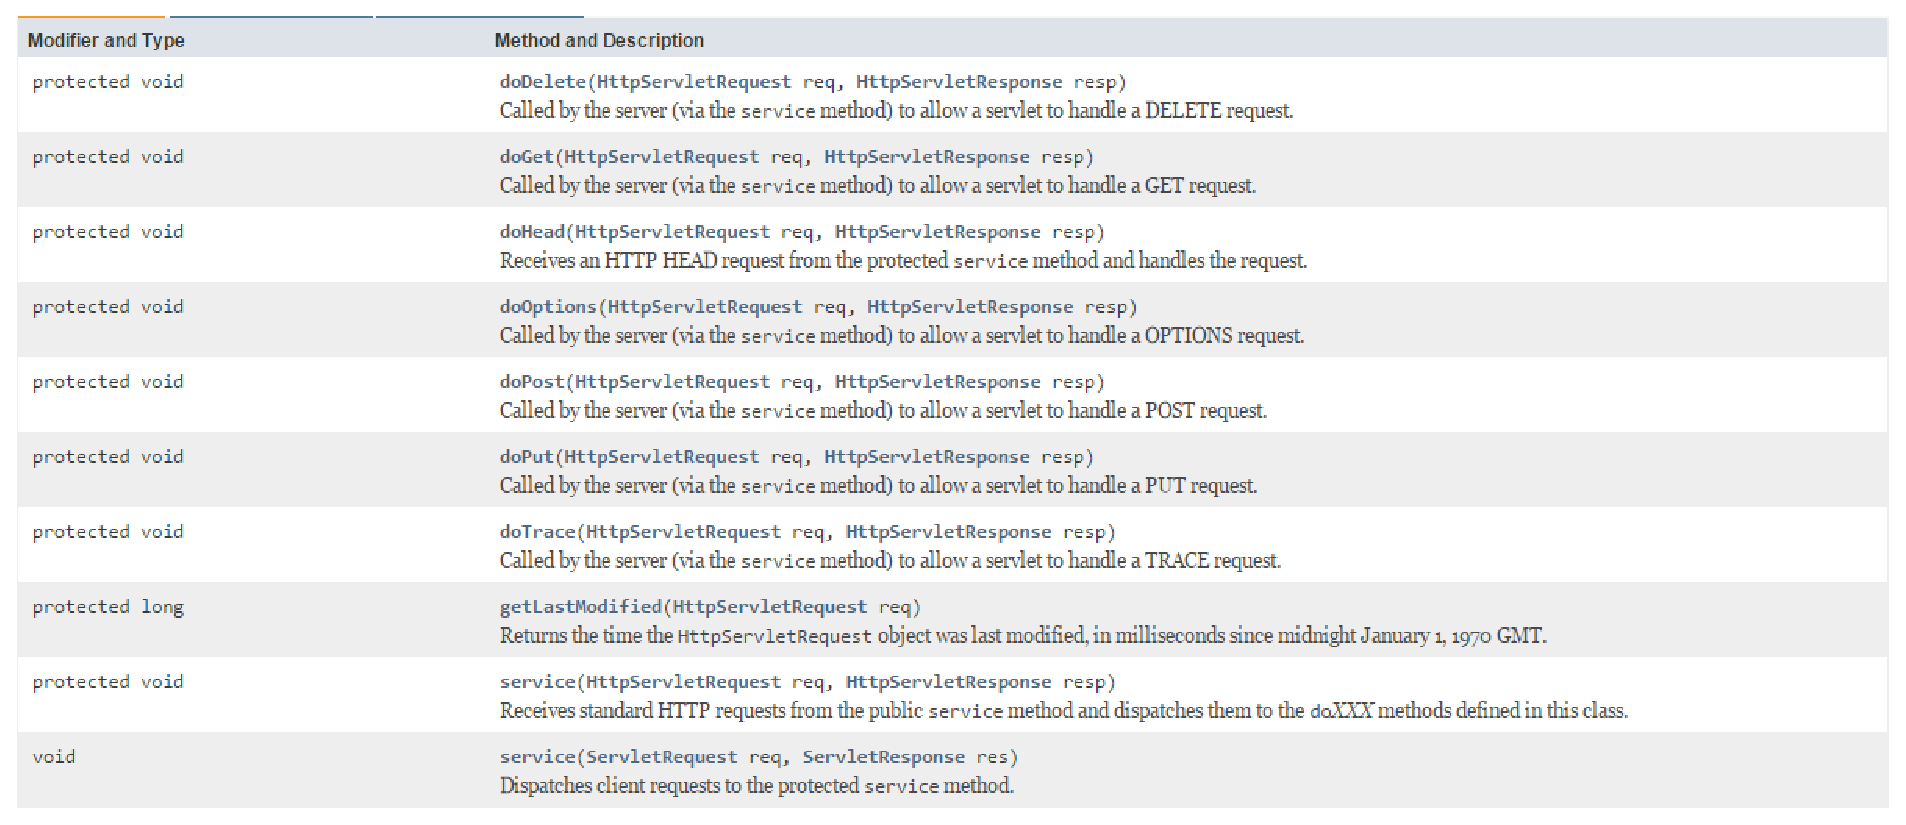
\includegraphics[keepaspectratio=true,scale=0.5]{figuras/httpservlet.eps}
	\fonte{\cite{httpservlet}.} 
\end{figure}

Os métodos mais utilizados são o \texttt{“doGet”} e \texttt{“doPost”} e serão os únicos que serão abordados neste trabalho. 
Eles funcionam de forma análoga aos métodos \textit{“GET”} e \textit{“POST”} empregados em conexões \texttt{HTTP}.
Um \texttt{Servlet} possui um ciclo de vida divido em três etapas: inicialização, execução e remoção. 
Primeiramente ele é carregado no servidor e permanece lá até que seja destruído. Após a inicialização, 
o \texttt{Servlet} estará apto a responder as requisições de usuários, etapa na qual caracteriza a sua execução. 
A etapa de remoção é utilizada para remover um \texttt{Servlet} do servidor, caso não seja removido ele permanecerá ocupando
espaço e processamento no servidor \cite[p.~21]{barale}.

\section{Tecnologias \textit{JSP} e \textit{JavaBeans}}

A tecnologia \texttt{Java Server Pages} permite gerar conteúdo da \textit{Web dinâmico}, como arquivos \texttt{DHTML}, \texttt{HTML}, \texttt{XHTML} e \texttt{XML}, que 
farão parte de uma aplicação para \textit{Web}. Uma página \texttt{JSP} consiste em uma codificação \texttt{HTML} mesclada com uma codificação 
\texttt{Java} inserida entre \textit{TAGS}. \texttt{JSP} faz parte da plataforma \texttt{J2EE (Java 2 Enterprise Edition)} e em conjunto com os \texttt{Java Servlets}
e \texttt{Java Beans} pode ser utilizado para desenvolver aplicações \textit{Web} eficientes, escaláveis e seguras. Esta tecnologia é importante 
principalmente por permitir que o programador separe conteúdos lógicos de conteúdos visuais, oferecendo uma melhor dinâmica de 
desenvolvimento. Além disso, ela permite a interação com os mais diversos tipos de bancos de dados existentes graças a 
tecnologia \texttt{JDBC (Java Database Connectiviy)} que será apresentada nos tópicos seguintes \cite[p.~3]{paulojsp}. Na \autoref{jsp} é apresentado um modelo 
minimalista de uma codificação na linguagem \texttt{JSP}.

\begin{figure}[h]
	\centering
	\caption{\label{jsp}Estrutura de um código \texttt{JSP}.}
		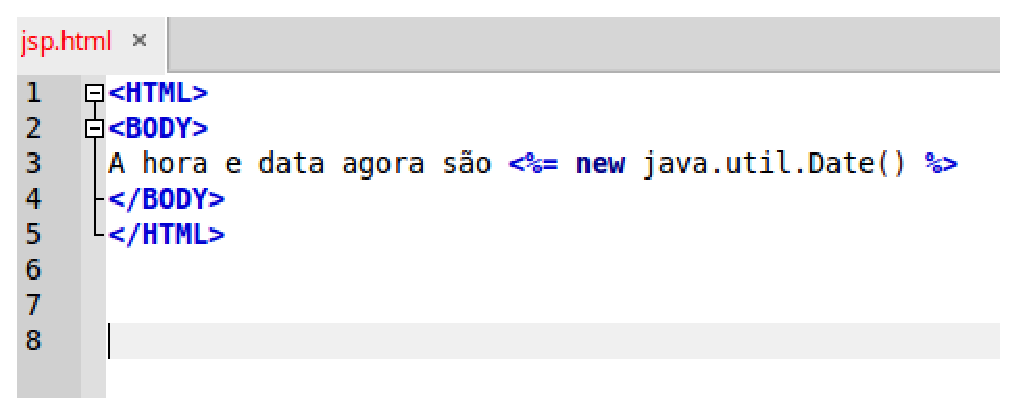
\includegraphics[keepaspectratio=true,scale=0.7]{figuras/jsp.eps}
	\fonte{Autoria própria.} 
\end{figure}

O autor \cite{paulojsp} descreve um \texttt{Bean} como uma classe em \texttt{Java} que segue um conjunto de convenções simples de \textit{design}
e nomeação determinado pela especificação \texttt{JavaBeans}. Para criar uma estrutura que obedece os conceitos de um \texttt{JavaBean} é necessário
seguir os seguintes passos:

\begin{itemize}

	\item O construtor de uma classe não deve receber argumentos;
	\item Podem existir diversos métodos públicos para determinar o valor de um atributo em um objeto. Esses métodos são chamados 
	de métodos \textit{setter};
	\item Podem existir diversos métodos públicos para obter o valor de um atributo em um objeto. Esses métodos são chamados de 
	métodos \textit{getter}.

\end{itemize}

A \autoref{bean1} apresenta como é implementada uma simples classe \texttt{JavaBean}.

\begin{figure}[h]
	\centering
	\caption{\label{bean1}Estrutura de um \texttt{JavaBean}.}
		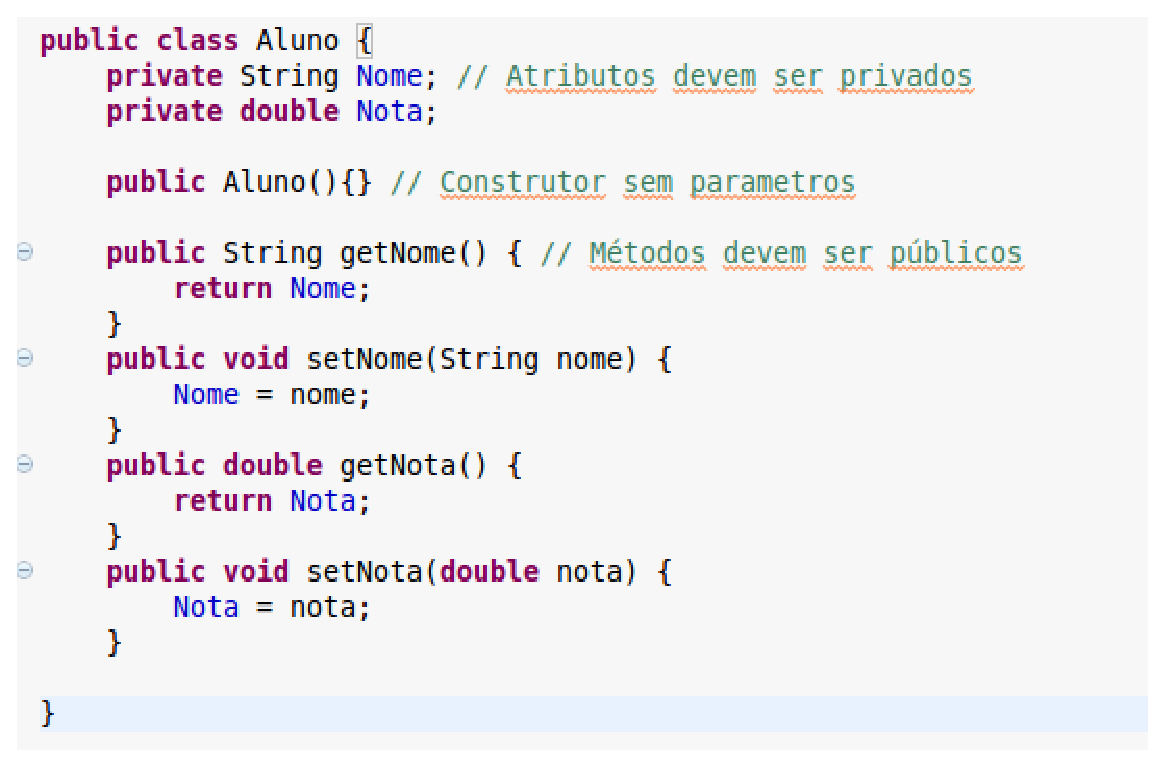
\includegraphics[keepaspectratio=true,scale=0.5]{figuras/bean1.eps}
	\fonte{Autoria própria.} 
\end{figure}

Por convenção e boa prática de programação, uma classe \texttt{JavaBean} precisa ter todos os seus atributos como privados e seus métodos \textit{“getters”} e \textit{“setters”}
como públicos. Além disso, é aconselhável que os métodos comecem com a primeira letra minúscula e colocar em maiúscula a primeira letra de 
cada palavra subsequente como apresenta a \autoref{bean2} \cite{paulojsp}.

\begin{figure}[h]
	\centering
	\caption{\label{bean2}Propriedades de um \texttt{JavaBean}.}
		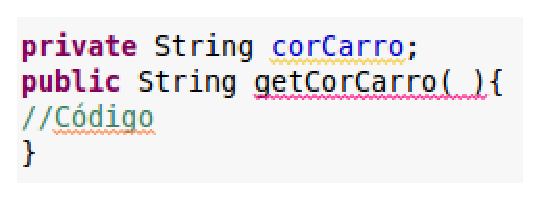
\includegraphics[keepaspectratio=true,scale=0.7]{figuras/bean2.eps}
	\fonte{Autoria própria.} 
\end{figure}

É importante destacar aqui a diferença entre \texttt{JavaBeans} e \texttt{EJB (Enterprise JavaBeans)}. A JavaBeans não tem o propósito de ser utilizado em 
componentes distribuídos como a \texttt{EJB} têm.

\section{Estrutura \textit{Model View Controller}}

A arquitetura de um sistema normalmente é composta de diversos elementos tais como, elementos de interação, elementos de conexão, elementos 
de persistência entre outros. Em sistemas de \textit{softwares} complexos a maneira como esses elementos se relacionam pode gerar dificuldades de 
implementação. Com o objetivo de padronizar a arquitetura de desenvolvimento de um \textit{software}, foi criado o modelo \texttt{Model View Controller (MVC)}.
O modelo \texttt{MVC} visa dividir uma aplicação em três partes: o modelo, a visão e o controlador \cite[p.~1]{devmediamvc}.

\begin{figure}[h]
	\centering
	\caption{\label{mvc}Modelo \texttt{MVC}.}
		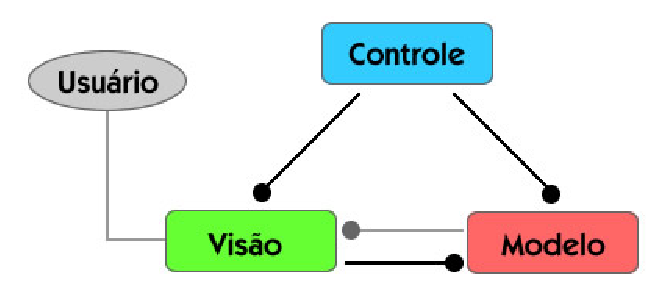
\includegraphics[keepaspectratio=true,scale=1]{figuras/mvc.eps}
	\fonte{\cite{mvc}.} 
\end{figure}

Explicando cada uma das partes do modelo \texttt{MVC} tem-se primeiramente o modelo \textit{(Model)} que é responsável pelo gerenciamento e acesso aos dados
que estão inclusos no banco de dados da aplicação. A visão \textit{(View)} é responsável pela interação entre o usuário e aplicação, é nela que os 
dados serão apresentados ao usuário. O controlador \textit{(Controller)} é responsável por delegar ao modelo as solicitações da visão. De forma geral
a visão recebe as informações do modelo, mas o modelo não tem conhecimento da visão. O responsável por essa comunicação é o controlador.

A principal ideia da arquitetura \texttt{MVC} é a separação dos códigos de forma organizada. O \texttt{MVC} é semelhante a clássica programação orientada a 
objetos e será de extrema importância neste trabalho. Entre as principais vantagens desta arquitetura é importante ressaltar a possibilidade de alteração de códigos contidos em qualquer 
uma das três partes sem gerar problemas nas partes adjacentes \cite{devmediamvc}.

\section{Estação de monitoramento - \textit{Software} de gerenciamento de dados e tomada de decisões}

A engenharia de \textit{software} terá um papel importante no desenvolvimento do sistema de
gerenciamento de dados \textit{Web}. Segundo \cite{falbo2005} a engenharia de \textit{software} surgiu
com o objetivo de melhorar a qualidade dos produtos de \textit{software} e aumentar a produtividade
no processo de desenvolvimento. A estratégia para aplicação dos conceitos de engenharia de
\textit{software} consiste na decomposição do problema original em partes menores. Esse método torna
possível a solução das partes decompostas, para posterior integração das soluções.

Com a crescente competitividade no ambiente empresarial, a eficiência de um sistema
está diretamente relacionada a sua qualidade. Segundo a NBR ISO 9000:2005, “qualidade é o
grau no qual um conjunto de características inerentes satisfaz aos requisitos”. Para o \textit{software}
apresentar um bom grau de qualidade, é necessário que a suas funcionalidades atendam de
forma eficaz todos os requisitos pré-estabelecidos.

Modelos podem ser utilizados para auxiliar a criação de um \textit{software}. O autor \cite{cole2011}
apresenta um exemplo de modelo cascata que foi uma das primeiras propostas para a
decomposição das etapas de um projeto, almejando a apresentação do projeto em sequência. A
simplicidade do modelo cascata facilita a explicação do projeto para pessoas que não estão
familiarizadas com o desenvolvimento de \textit{software}. A \autoref{cascata} apresenta como funciona o modelo
em cascata.

\begin{figure}[h]
	\centering
	\caption{\label{cascata}Modelo Cascata Puro utilizado no desenvolvimento de \texttt{softwares}.}
		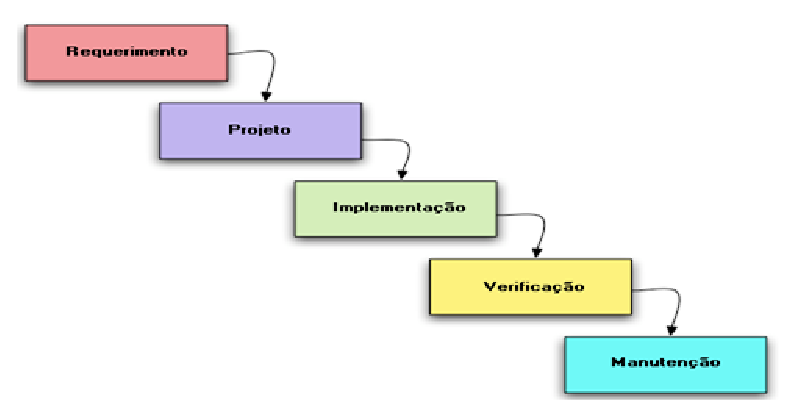
\includegraphics[keepaspectratio=true,scale=1]{figuras/cascata.eps}
	\fonte{\cite{cole2011}.} % Referencia errada
\end{figure}

Ainda segundo \cite{cole2011}, na fase de requerimentos são estabelecidos os
requisitos do sistema a ser desenvolvido. Esta etapa também pode ser chamada de engenharia
de requisitos, em que é feita a modelagem conceitual do sistema. A etapa de projeto tem como
objetivo definir como serão atingidos os requerimentos estabelecidos, de modo que o conjunto
de informações adquiridas permita o início da etapa de implementação. Na fase de
implementação o programa começa a ser estruturado e codificado. A base de dados também é
criada e todos os módulos que compõe o projeto são interligados. Após o término da fase de
implementação é iniciada a etapa de verificação, que consiste na realização de diversos testes
sob o sistema projetado. Estes testes tem como objetivo encontrar erros e inconsistências na
utilização do \textit{software}. Com o \textit{software} concluído e entregue a empresa, é iniciada a etapa de
manutenção. A etapa de manutenção consiste em oferecer suporte a empresa caso problemas
ou erros sejam encontrados pela empresa.

O desenvolvimento de sistemas que utilizam conceitos de orientação a objetos nas fases de análise de requisitos,
análise de sistemas e \textit{design} não oferecia uma notação padrão específica e eficaz que guiasse no projeto de tais sistemas.
Existem diversas simbologias e cada uma com seus próprios conceitos. Visando resolver tal problema, foi criado por um grupo 
de amigos entusiastas da área de modelagem orientada a objetos, a \texttt{“Unified Modeling Language” (UML)}. A \texttt{UML} é uma padronização 
de notação na parte de modelagem orientada a objetos. Essa padronização visava a modelagem de sistemas (não apenas de \textit{software}) 
que utilizavam dos conceitos de orientação a objetos, a união de métodos conceituais com executáveis e a criação de uma linguagem 
de modelagem usável tanto pelo homem como por uma máquina. Seu principal objetivo é descrever qualquer sistema em termos de diagramas 
orientado a objetos \cite{uml}.

Ainda segundo a apostila \cite{uml} que descreve a \texttt{UML} como a composição de 4 componentes que estão apresentados abaixo:

\begin{itemize}

	\item Visões: A visão é um conjunto de diagramas que mostram os diferentes aspectos de um sistema que está sendo modelado;
	\item Modelos de elementos: Representam definições comuns da orientação a objetos como as classes, objetos, mensagem, 
	relacionamento entre classes incluindo associações, dependências e heranças;
	\item Mecanismos gerais: Provém comentários suplementares, informações, ou semântica sobre os elementos que compõe o modelo;
	\item Diagramas: Os diagramas são os gráficos que descrevem o conteúdo em uma visão.

\end{itemize}

Os diagramas utilizados pela \texttt{UML} são compostos por nove tipos: diagramas de caso de uso, de classes, de objetos, de estado, de sequência,
de colaboração, de atividade, de componente e o de execução.

O diagrama de casos de uso descreve o comportamento do sistema de uma forma geral. Nele são especificados argumentos funcionais que 
determinarão a arquitetura geral do sistema. Para a \texttt{UML} um requisito normalmente é uma funcionalidade desejada do sistema. 
O diagrama de casos de uso é responsável por detalhar os requisitos solicitados. Todas as funções especificas do sistema identificadas 
na fase de requisitos devem se tornar casos de uso.

O diagrama de classes é utilizado na modelagem estrutural de um sistema orientado a objetos. Este diagrama é considerado estático pois 
a estrutura descrita é sempre válida em qualquer ponto do ciclo de vida do sistema. As classes possuem atributos, operações e associações 
entre outras classes. Todas estas peculiaridades estão inclusas em um diagrama de classe. Sistemas podem possuir um ou mais diagramas de
classe, já que não são todas as classes que se relacionam.

O diagrama de objetos é utilizado para mapear a relação entre os objetos de cada classe. É muito semelhante ao diagrama de classes, 
porém é composto de instancias que possuem os valores dos atributos dos objetos. Normalmente são utilizados na validação de um diagrama 
de classes ou identificação de problemas na execução de uma aplicação.

O diagrama de estado é responsável por descrever o comportamento de objetos em relação a eventos. Ele apresenta o ciclo de vida de um objeto 
mostrando os eventos que causam a transição de um estado para outro estado e as ações que resultam de uma mudança de estado. Este diagrama
não é escrito para todas as classes de um sistema e sim somente para aquelas que possuem um número definido de estados conhecidos e onde o 
comportamento das classes é afetado pelos diferentes estados.

O diagrama de sequência é responsável por apresentar a colaboração dinâmica entre os objetos de um sistema. Sua principal característica é 
a possibilidade de visualização da sequência de mensagens trocadas entre os objetos.

O diagrama de colaboração é semelhante ao diagrama de sequência. No diagrama de colaboração também estão inclusos os relacionamentos entre
os objetos. Normalmente pode-se escolher entre utilizar o diagrama de colaboração ou o diagrama de sequência.

O diagrama de atividades permite descrever as operações associadas a um objeto e também suas interações com outros objetos. Este diagrama 
é uma variação do diagrama de estado com o objetivo de capturar ações e seus resultados em termos de mudanças de estados dos objetos. 

O diagrama de componente e de execução tem como objetivo mostrar o lado funcional do sistema, descrevendo a relação entre seus componentes 
e organização de seus módulos durante sua execução. O diagrama de componentes mostra a organização estrutural de todo o código gerado para
aplicação. Já o diagrama de execução apresenta a arquitetura física do \textit{hardware} e do \textit{software} do sistema, incluindo diversos periféricos, 
computadores e as conexões estabelecidas entre eles.

Como já apresentado, a importância da informática na gestão das empresas é inquestionável. As
empresas ganham agilidade, confiabilidade e ainda podem reduzir seus custos se o
gerenciamento for feito de forma eficaz. Para se obter um gerenciamento eficaz, é necessário
ter um \textit{software} que forneça dados consistentes e de forma organizada. A \cite{sbsistemas2015}
destaca como a utilização de um \textit{software} de gestão pode auxiliar na tomada de decisões,
organização de planejamento estratégico e ainda descobrir quais áreas da empresa precisam de
maior atenção. Além de todas essas vantagens, um \textit{software} de gestão oferece a possibilidade
de gerenciamento de permissões de acesso, assim é possível controlar o que cada funcionário 
tem acesso. O sistema a ser desenvolvido neste projeto, contará com esse gerenciamento de
permissões de acesso. Os funcionários não terão acesso as funções dos administradores.

\section{Banco de dados e \textit{driver JDBC}}

Em muitos sistemas computacionais o banco de dados pode ser considerado como a parte mais
importante da aplicação, o sucesso do sistema está totalmente relacionado com o bom
funcionamento do banco de dados, conforme descreve  \cite{marcilio2004}. No projeto em questão o banco de
dados terá papel fundamental no armazenamento de tabelas, relatórios e/ou dados que possam
auxiliar no processo de gerenciamento da empresa.

Um banco de dados pode ser definido como uma coleção de dados organizados de forma sistemática. Esses dados são acessados e gerenciados por
um \texttt{Sistema de Gerenciamento de Banco de Dados (SGBD)}. O sistema de gerenciamento provê mecanismos de organização, recuperação, 
alteração e armazenagem de dados. As consultas em bancos de dados relacionais são realizadas em uma linguagem de padrão internacional 
conhecida como \texttt{SQL} \cite{bdrelacional}.O processo de funcionamento de um \texttt{SGBD} é apresentado de forma sucinta por \cite[p.~2]{marcilio2004}:


\begin{citacao}
 
 ''Aplicações que utilizam \texttt{SGBDs} para gerenciar dados executam processos separados para conectar com o \texttt{SGBD}.
 Uma vez que uma conexão é estabelecida, comandos \texttt{SQL} podem ser usados para inserir, apagar ou modificar dados. 
 Consultas \texttt{SQL} podem ser usadas para restaurar dados desejados, mas, mas é necessário exibir uma importante diferença
 de como o sistema de banco de dados “vê” os dados e como uma aplicação desenvolvida em linguagens como \texttt{C++} ou \texttt{Java} vêem 
 os dados: o resultado de uma consulta no banco de dados é um conjunto (ou coleção) de registros, mas linguagens estruturadas 
 com \texttt{Java}, por exemplo, não possui um tipo de dado correspondente. Esta “falta de combinação”, conhecida como \textit{impedance mismatch}, 
 entre as linguagens é resolvida através de construções adicionais \texttt{SQL} que possibilitam às aplicações reconhecer e acessar um conjunto 
 e interagir com um registro por vez.``
  
 \end{citacao}

Alguns dos sistemas de gerenciamento de banco de dados mais utilizados no mundo são: \texttt{Microsoft SQL Server}, \texttt{Oracle}, \texttt{MySQL} e \texttt{PostgreSQL}.
Neste trabalho o sistema de gerenciamento a ser utilizado será o PostgreSQL.

O livro \cite[p.~900]{deitel2009java} descreve um banco de dados relacional como uma representação lógica de dados, que permite que os dados sejam acessados sem considerar sua estrutura física. Os dados em um banco de dados são armazenados no formato de tabelas.

 Existem duas principais formas de se armazenar dados atualmente, a primeira delas é fazendo o uso de arquivos de dados permanentes e a 
 segunda é a utilização de um banco de dados. O banco de dados apresenta inúmeras vantagens em relação a um sistema de arquivos como: a 
 centralização dos dados, eliminação de inconsistências, controle de redundância, independência de dados e facilidade de acesso \cite{bdrelacional}. 
 
 A centralização dos dados ocorre pelo fato de todos os dados estarem concentrados em um único local, já no sistema de arquivos cada 
 aplicação mantém seus próprios arquivos. 

 A garantia da integridade em um banco de dados está diretamente relacionada a consistência dos dados. Em um sistema de arquivos pode 
 ocorrer a repetição da informação armazenada fazendo com que um mesmo dado apresente valores diferentes dependendo de como esses arquivos
 são acessados. Em um banco de dados o mesmo não ocorre garantindo a integridade das informações e a consistência dos dados.
 
 Em um sistema de arquivos geralmente uma mesma informação pode estar presente em um ou mais arquivos, causando um desperdício de espaço 
 de armazenamento. No banco de dados, o dado é armazenado apenas uma vez e pode ser compartilhado por diversos usuários evitando assim a 
 redundância.
 
 A definição da estrutura de armazenamento e do método de acesso aos dados em um sistema de arquivos, está inclusa no código da aplicação.
 Para fazer quaisquer alterações nas definições ou métodos de acesso, é necessário modificar a aplicação, gerando mais trabalho e consumindo
 mais tempo. No banco de dados o mesmo não ocorre, pois, os dados são independentes da aplicação. Este fato recebe o nome de abstração de 
 dados.

 O processo de armazenamento dos dados também é conhecido como persistência. Em \texttt{Java} a biblioteca padrão de persistência em um banco de dados
 relacional recebe o nome de \texttt{JDBC (Java Database Connectivity)}. Com o objetivo de evitar que cada banco de dados tenha sua \texttt{API}, conjunto 
 de classes e métodos, existe um único conjunto de interfaces muito bem definidas. Este conjunto de interfaces é representado como um \textit{driver}
 (\texttt{JDBC}). Normalmente os sistemas de gerenciamento de banco de dados fornecem seus \textit{drivers} \cite{caelumweb}.
 
 Entre as inúmeras interfaces deste pacote pode-se destacar a \texttt{“Connection”}. Esta e outras interfaces são responsáveis por fazer a ponte entre 
 o código do cliente que usa a \texttt{API JDBC} e o banco de dados, como mostra a \autoref{jdbc}.
 
 \begin{figure}[h]
	\centering
	\caption{\label{jdbc}Interação entre o banco de dados e o cliente.}
		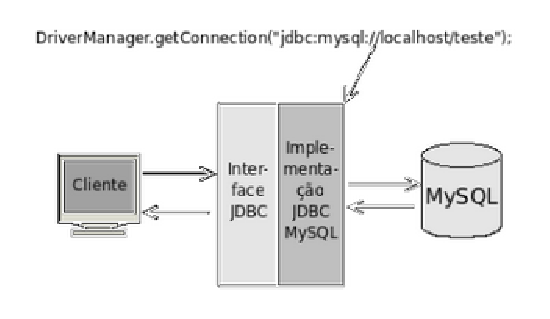
\includegraphics[keepaspectratio=true,scale=1]{figuras/jdbc.eps}
	\fonte{\cite{caelumweb}.} % Referencia errada
\end{figure}
 
 \section{A linguagem \textit{CSS}}
 
 Quando a linguagem \texttt{HTML} surgiu, seu objetivo era apenas de mostrar um determinado conteúdo para um usuário, sem se preocupar com a formatação
 e apresentação dos dados na tela. A medida em que o tempo passou, surgiram novas necessidades de formatação e apresentação de dados relacionadas
 a linguagem \texttt{HTML}. A própria linguagem \texttt{HTML} passou a ser utilizada para o controle da aparência do documento tornando a linguagem mais complexa 
 conforme descreve \cite{isabelecss}.
 
 No ano de 1994, um desenvolvedor chamado de \texttt{Hakon Lie} propôs a criação da linguagem \texttt{CSS (Cascade Style Sheets)}. A \texttt{CSS} é uma linguagem de 
 estilos utilizada para definir a apresentação de documentos escritos em uma linguagem de marcação, como \texttt{HTML} e \texttt{XML}. Com o surgimento da 
 \texttt{CSS}, os códigos \texttt{HTML} passaram a ter \textit{links} (ligação) para um arquivo \texttt{CSS} que contém os estilos de uma respectiva página \texttt{HTML}. Com isso 
 foi possível separar o formato de uma página \texttt{HTML} de seu conteúdo, tornando assim o código mais organizado, funcional e simples \cite{isabelecss}.
 
 A utilização da linguagem \texttt{CSS} na definição de estilos de páginas \texttt{HTML} apresenta algumas vantagens como:
 
 \begin{itemize}

	\item Controle de \textit{layout} de vários documentos partir de um único arquivo \texttt{CSS};
	\item Facilidade de implementação por ser estruturado em classes;
	\item Rapidez por ter a possibilidade de utilizar apenas uma classe para muitos documentos, diminuindo assim conteúdo desnecessário;
	\item Boa portabilidade por funcionar em qualquer navegador;
	\item Precisão no controle do \textit{layout}.

\end{itemize}

Neste projeto a linguagem \texttt{CSS} terá papel fundamental na criação da interface, objetivando proporcionar ao usuário uma experiência simples 
e agradável de navegação no sistema \textit{Web}.

\section{Ferramentas de Desenvolvimento}

Para o desenvolvimento de um sistema \textit{Web} completo, incluindo banco de dados, servidor \textit{Web}, periféricos e aplicação \texttt{Java} \textit{Web},
é necessário a utilização de algumas ferramentas. Estas ferramentas são \textit{softwares} que tem como 
objetivo tornar o desenvolvimento rápido, seguro e eficiente.

Entre tais ferramentas estão inclusas ambientes integrados de desenvolvimento, \textit{plug-ins} e alguns \textit{softwares}. Nas próximas seções serão
apresentadas as ferramentas utiliadas no desenvolvimento deste projeto.

\subsection{Ferramenta de desenvolvimento - \textit{Eclipse IDE}}

O \texttt{Eclipse} é uma \texttt{IDE (Integrated Development Environment)} baseada em \texttt{Java} líder de mercado. Formada por um consórcio de empresas
lideradas pela \texttt{IBM} possui seu código livre. Esta \texttt{IDE} compreende os mais diversos tipos de linguagens como \texttt{Java}, \texttt{C/C++}, \texttt{PHP}, \texttt{Python}, 
\texttt{Pearl} e ainda aceita a instalação de \textit{plug-ins} que auxiliam no desenvolvimento de aplicações.

O principal diferencial do \texttt{Eclipse} é apresentado segundo \cite{augustoeclipse}:

\begin{citacao}

 '' O grande diferencial do \texttt{Eclipse} é a sua neutralidade em relação à linguagem de programação e ao sistema operacional. 
 O \texttt{Eclipse Consortium}, formado pela \texttt{IBM}, \texttt{Merant}, \texttt{HP}, \texttt{Borland}, \texttt{Fujitsu}, \texttt{Red Hat}, \texttt{Sybase}, \texttt{Oracle}, \texttt{Rational} e outras dezenas 
 de empresas e organizações, fornece suporte a \texttt{Java}, \texttt{C} e \texttt{COBOL} nas plataformas \texttt{Windows}, \texttt{Linux}, \texttt{AIX}, \texttt{Solaris}, \texttt{HP-UX}, \texttt{QNX} e
 \texttt{MacOS}. Mas, como o \textit{framework} é livre, qualquer um pode adicionar o suporte a seu ambiente preferido, e já existem mais de 
 260 \textit{plug-ins} para o \texttt{Eclipse} disponíveis no \texttt{SourceForge} e outros sites para desenvolvedores \texttt{Perl}, \texttt{Python}, \texttt{Pascal}, \texttt{PHP} e até \texttt{Clipper}.``
 
\end{citacao}

Pelo fato do \texttt{Eclipse} ter sido escrito em \texttt{Java}, é necessário ter uma máquina virtual \texttt{Java (JRE)} para rodá-lo, por este fato surge 
sua independência do sistema operacional.
Para facilitar o desenvolvimento \textit{Web} será utilizado uma plataforma chamada \texttt{Web Tools Plataform (WTP)}. Esta plataforma é um 
conjunto de \textit{plug-ins} que têm como objetivo tornar o desenvolvimento de aplicações \texttt{Java EE} mais atrativas. Neste pacote estão 
inclusos editores para as linguagens que serão utilizadas neste projeto como \texttt{JSP}, \texttt{CSS}, \texttt{HTML} e \texttt{Java}. Existe uma versão do \texttt{Eclipse} 
(\texttt{Eclipse IDE for Java EE Developers)} que já vêm com esse \textit{plug-in} em sua versão padrão. A \autoref{eclipse} apresenta a interface do \texttt{Eclipse IDE
for Java EE Developers}.

 \begin{figure}[h]
	\centering
	\caption{\label{eclipse}Interface da \texttt{Eclipse IDE}.}
		\includegraphics[keepaspectratio=true,scale=0.3]{figuras/eclipse.eps}
	\fonte{Autoria própria.} % Referencia errada
\end{figure}

\subsection{Servidor \textit{Web - Apache Tomcat}}

O \texttt{Apache Tomcat} é um servidor \texttt{Java} \textit{Web} desenvolvido pela \texttt{Apache Software Foundation}. É um \textit{software} livre que têm como habilidade 
converter páginas \texttt{JSP} em um \texttt{Servlet}. Pode-se dizer que ele gera códigos em \texttt{Java} a partir de códigos em \texttt{HTML} como apresenta \cite{devmediatomcat}.

O autor \cite{flaviocoutinho} define o \texttt{Tomcat} como sendo “é um \texttt{Servlet} \textit{Container}, ou seja, é um servidor onde são instaladas \texttt{Servlets} 
para tratar as requisições que o servidor receber”.

A dinâmica do funcionamento de um processo de acesso à páginas \textit{Web} segue a seguinte lógica: primeiramente o usuário faz uma solicitação 
de uma página indicada por meio de uma \texttt{URL} no \textit{browser}; o servidor \texttt{Apache Tomcat} recebe a solicitação do usuário, executa o \texttt{Servlet} ou \texttt{JSP} 
associado a respectiva \texttt{URL} e então, o conteúdo gerado pelo \texttt{Servlet} ou \texttt{JSP} é apresentado no formato \texttt{HTML}; por fim, o usuário recebe o 
conteúdo gerado pelo \texttt{Tomcat} em seu \textit{browser} \cite{devmediatomcat}.


\subsection{Sistema de Gerenciamento de banco de dados - \textit{PostgreSQL}}

O sistema gerenciador de banco de dados \texttt{PostgreSQL} surgiu na \texttt{Universidade de Berkeley}, na Califórnia, em 1986.  Um desenvolvedor de nome 
\texttt{Michael Stonebraker} foi responsável por liderar uma equipe de desenvolvimento para criação de um banco de dados relacional. Surgiu então 
a primeira versão de um banco de dados relacional, chamada de \texttt{Postgres}. Posteriormente dois estudantes de \texttt{Berkeley} incorporaram a linguagem 
\texttt{SQL} ao \texttt{Postgres}, dando origem ao \texttt{Postgres95}. Em 1996 uma nova versão foi lançada definindo a linguagem \texttt{SQL} como padrão, esta versão recebeu
o nome de \texttt{PostgresSQL} conforme explica \cite{emersonalecrim}. 

O \texttt{PostgreSQL} é gratuito e possui seu código aberto. Atualmente é um banco de dados que suporta a maior quantidade de arquiteturas e \textit{software} 
do mercado, além de possuir uma comunidade de suporte a assuntos relacionados ao \texttt{PostgreSQL} \cite{postgrelinux}. Normalmente é utilizado em 
aplicações complexas com grande volume de dados como discute \cite{emersonalecrim}. 

\subsection{Ferramenta de gerenciamento do \textit{PostgreSQL - pgAdmin}}
 
 Para realizar a administração do banco de dados de uma maneira mais eficiente, será utilizada uma ferramenta \texttt{pgAdmin}.
 Esta ferramenta proporciona um ambiente visual gráfico de administração do sistema gerenciador de banco de dados \texttt{PostgreSQL}. 
 Foi desenvolvida pela própria equipe de desenvolvimento do \texttt{PostgreSQL}.
